%latex model.tex
%bibtex model
%latex model.tex
%latex model.tex
%pdflatex model.tex

%se poate lucra si online (de ex www.overleaf.com)


\documentclass[twoside,runningheads,a4paper,11pt]{report}

\usepackage{algorithmic}
\usepackage{algorithm} 
\usepackage{array}
\usepackage{amsmath}
\usepackage{amsfonts}
\usepackage{amssymb}
\usepackage{amsthm}
\usepackage{caption}
\usepackage{comment} 
\usepackage{epsfig} 
\usepackage{fancyhdr}
\usepackage[T1]{fontenc}
\usepackage{geometry} 
\usepackage{graphicx}
\usepackage[colorlinks]{hyperref} 
\usepackage[latin1]{inputenc}
\usepackage{multicol}
\usepackage{multirow} 
\usepackage{rotating}
\usepackage{setspace}
\usepackage{subfigure}
\usepackage{url}
\usepackage{verbatim}
\usepackage{xcolor}

\geometry{a4paper,top=3cm,left=2cm,right=2cm,bottom=3cm}

\pagestyle{fancy}
\fancyhf{}
\fancyhead[LE,RO]{Project's name}
\fancyhead[RE,LO]{Team's name}
\fancyfoot[RE,LO]{MIRPR 2025-2026}
\fancyfoot[LE,RO]{\thepage}

\renewcommand{\headrulewidth}{2pt}
\renewcommand{\footrulewidth}{1pt}
\renewcommand{\headrule}{\hbox to\headwidth{%
  \color{lime}\leaders\hrule height \headrulewidth\hfill}}
\renewcommand{\footrule}{\hbox to\headwidth{%
  \color{lime}\leaders\hrule height \footrulewidth\hfill}}

\hypersetup{
pdftitle={artTitle},
pdfauthor={name},
pdfkeywords={pdf, latex, tex, ps2pdf, dvipdfm, pdflatex},
bookmarksnumbered,
pdfstartview={FitH},
urlcolor=cyan,
colorlinks=true,
linkcolor=red,
citecolor=green,
}
% \pagestyle{plain}

\setcounter{secnumdepth}{3}
\setcounter{tocdepth}{3}

\linespread{1}

% \pagestyle{myheadings}

\makeindex


\begin{document}

\begin{titlepage}
\sloppy

\begin{center}
BABE\c S BOLYAI UNIVERSITY, CLUJ NAPOCA, ROM\^ ANIA

FACULTY OF MATHEMATICS AND COMPUTER SCIENCE

\vspace{6cm}

\Huge \textbf{Project RIBS}

\vspace{1cm}

\normalsize -- MIRPR report --

\end{center}


\vspace{5cm}

\begin{flushright}
\Large{\textbf{Team members}}\\
Alexandra-Cristina Pu\c sca\c s, Computer Science\\
Bianca-Gabriela Pulp\u a, Computer Science\\
Bogdan-C\u alin-Florin Rebele\c s, Computer Science\\
\end{flushright}

\vspace{4cm}

\begin{center}
2025-2026
\end{center}

\end{titlepage}

\pagenumbering{gobble}

\begin{abstract}
This report investigates a multi-biomarker "virtual biopsy" approach for non-small cell lung cancer (NSCLC), aiming to build models that can predict several tumor biomarkers simultaneously from medical imaging. The motivation is that biomarker determination often depends on tissue biopsy, which is invasive and may be challenging or infeasible in some clinical scenarios. We explore hybrid strategies that combine deep learning (features learned from CT/PET volumes) with radiomics (and optionally basic patient metadata) to estimate biomarker likelihood for targets such as TTF1, NAPSIN, and CK7.

The dataset comprises 101 patients with paired CT+PET imaging and biopsy-confirmed labels. Experiments cover both pilot settings (e.g., small cohorts) and larger subsets, using preprocessing steps such as segmentation-based cropping and normalization, and evaluating 3D architectures including multimodal variants (e.g., 3D ResNet-based models) as well as 2D slice-based architectures (e.g., EfficientNet-based models). Overall performance is modest under limited-data conditions, highlighting the impact of ROI definition/cropping and the potential utility of radiomic descriptors, while also underlining the need for larger and more diverse cohorts to achieve clinically robust generalization.
\end{abstract}


\tableofcontents

\newpage

\listoftables
\listoffigures
\listofalgorithms

\newpage

\setstretch{1.5}

\newpage

\pagenumbering{arabic}


\chapter{Introduction}
\label{chapter:introduction}

\section{What? Why? How?}
\label{section:what}

Lung cancer remains one of the most severe oncological diseases, and the management of non-small cell lung cancer (NSCLC) increasingly relies on tumor biomarkers that guide diagnosis, prognosis, and therapy selection. In current clinical workflows, many clinically relevant biomarkers (e.g., immunohistochemical and genomic markers) are determined using tissue biopsy, which can be invasive, costly, and sometimes impractical for patients with advanced disease or limited lesion accessibility. Consequently, there is a strong need for methods that can provide biomarker information non-invasively, early, and at scale.

The scientific problem addressed in this project is the automated prediction of multiple NSCLC tumor biomarkers directly from medical imaging, aiming to build a "virtual biopsy" system that can estimate biomarker likelihood from imaging phenotypes. The clinical motivation is clear: a reliable image-based predictor could reduce dependency on invasive procedures, support faster decision-making, and complement pathological testing by providing an additional source of evidence for personalized treatment strategies. The intended users are radiologists, oncologists, and clinical researchers, for whom such a tool could act as a decision-support component in diagnostic and treatment planning workflows.

Our basic approach is to combine deep learning representations with radiomics features (and, when available, basic patient metadata), leveraging complementary strengths: deep models can learn complex imaging patterns, while radiomics provides interpretable quantitative descriptors that often remain robust in small-data regimes. The dataset described in this report includes NSCLC cases with paired CT/PET imaging and biopsy-confirmed biomarker labels (e.g., TTF1, NAPSIN, CK7), which enables supervised learning and objective evaluation.

This work is positioned in the context of recent research showing that radiomics and multimodal deep learning can non-invasively predict clinically meaningful biomarker status (e.g., PD-L1 and oncogene mutations), especially when CT and PET information are fused and/or combined with clinical variables. Building on these directions, we investigate multiple architectures and fusion strategies, and we evaluate them using standard classification metrics such as AUC, sensitivity, specificity, and F1-score.

The objectives of this report are therefore: (1) to formalize the "virtual biopsy" task for multi-biomarker prediction in NSCLC using imaging data; (2) to develop and compare several model families (radiomics-only baselines, 3D CNNs, and hybrid deep learning + radiomics models); and (3) to outline how these models can be integrated into an application-oriented workflow. The experimental results presented in the investigated approaches highlight both the potential and the practical challenges of small clinical datasets: radiomics-only models may remain competitive when data are scarce, while hybrid and deep models require careful design and validation to generalize reliably. 


\section{Paper structure and original contribution(s)}
\label{section:structure}

The research presented in this report advances the design and implementation of several predictive models for non-invasive biomarker estimation in NSCLC, with a focus on hybrid learning strategies that combine radiomics and deep imaging features.

The main contribution of this report is the development and evaluation of an intelligent algorithmic pipeline for solving the problem of automated, non-invasive prediction of \textbf{multiple} lung cancer biomarkers from medical imaging (CT/PET), using biopsy-confirmed labels as ground truth and reporting standard quantitative metrics for performance assessment.

The second contribution consists of a systematic experimental study that compares multiple modeling strategies under realistic constraints (limited cohort sizes and multi-label/multi-class outputs), including:
\begin{itemize}
    \item deep learning models operating on 3D volumes,
    \item radiomics-only and ct-only machine learning baselines,
    \item hybrid architectures that fuse deep features with selected radiomic descriptors to improve robustness and generalization on small datasets.
\end{itemize}

\chapter{Scientific Problem}
\label{section:scientificProblem}
The problem addressed in this project is the automated, non-invasive prediction of multiple tumor biomarkers in patients diagnosed with non-small cell lung cancer (NSCLC) using medical imaging data. In current clinical practice, biomarker evaluation, such as immunohistochemical (IHC) and genomic markers, is typically performed through tissue biopsies, which are invasive, expensive, and sometimes unfeasible for patients with advanced or inoperable disease. This project aims to develop an artificial intelligence (AI) model that can predict several clinically relevant tumor biomarkers directly from imaging data, using a hybrid approach that combines radiomics, deep learning, and patient-level demographic information.

This problem is of major clinical importance because accurate identification of tumor biomarkers guides personalized treatment strategies, including targeted therapies and immunotherapy. A reliable, non-invasive AI system would reduce the dependence on tissue biopsies, minimize patient risk, and enable faster, more accessible screening for actionable molecular markers. Such a tool could play a transformative role in precision oncology by providing physicians with immediate diagnostic insights before biopsy results are available.

The intended users of this AI system are radiologists, oncologists, and clinical researchers, who can use the tool as a decision-support system to complement manual image interpretation and laboratory tests. It is designed to assist in both diagnostic and treatment planning workflows by highlighting potential biomarker profiles based on imaging phenotypes.

The dataset used in this study consists of medical imaging data from 101 patients diagnosed with NSCLC, each having paired CT (Computed Tomography) and PET (Positron Emission Tomography) scans, with an average slice thickness of approximately 3.8 mm for CT and 3.3 mm for PET. All patients also underwent tissue biopsy, which provides the ground-truth labels for the corresponding tumor biomarkers used in training and validation. The cohort includes 42 female and 59 male patients, and the imaging data are stored in standard DICOM format. The paired multimodal volumes, optionally supplemented with basic clinical metadata such as patient age or sex, are processed through an AI pipeline that performs image preprocessing, feature extraction (radiomics and deep features), and predictive modeling. The output of the system is a set of predictions indicating the likelihood of the presence or expression level of multiple tumor biomarkers, such as TTF1, NAPSIN, and CK7, each represented as a confidence score or classification label. \cite{Shao2022-yo} This comprehensive dataset, together with biopsy-confirmed biomarker status, provides a solid foundation for developing and evaluating fusion-based deep learning models, allowing the system to learn complementary metabolic and anatomical signatures relevant for biomarker prediction.


To explore the impact of multimodal fusion strategies, we will develop three separate AI models that all rely on DenseNet-based feature extractors, but differ in how PET and CT information is combined. The first model will use early fusion, merging the modalities at the input or initial feature-map level. The second will use intermediate (late) fusion, combining deep features only after several DenseNet blocks. The third model will also follow a late fusion design, but with shared convolutional weights between the PET and CT pathways, ensuring that both modalities learn synchronized feature representations. This setup allows a systematic comparison of fusion mechanisms while maintaining architectural consistency across models.~\cite{Da-Ano2024-oo} In all three cases, the fused deep features will be further combined with radiomic features at the decision stage, enabling a hybrid prediction mechanism that leverages both learned representations and quantitative imaging biomarkers.~\cite{Li2024-np}


Model performance is evaluated quantitatively using standard classification and regression metrics, depending on the biomarker type. The main metrics include the AUC, sensitivity, specificity, and F1-score. Cross-validation on the training data and testing on independent validation cohorts are applied to ensure the robustness, generalizability, and clinical reliability of the model. 

Overall, the project seeks to create a clinically interpretable, reproducible, and data-driven virtual biopsy system capable of predicting multiple tumor biomarkers from PET/CT imaging, thus contributing to the ongoing shift toward precision medicine in lung cancer management.



\chapter{State of the art/Related work}
\label{chapter:stateOfArt}

\section{Automated PD-L1 status prediction in lung cancer with multi-modal PET/CT fusion}
Da-Ano et al. (2024) developed a deep learning framework for non-invasive prediction of PD-L1 expression in non-small cell lung cancer (NSCLC) using multi-modal positron emission tomography/computed tomography (PET/CT) imaging \cite{Da-Ano2024-oo}. The study included 189 NSCLC patients from a single clinical center in France, each having both PET and CT scans acquired on Siemens Biograph mCT40 systems. The aim was to replace invasive biopsy-based immunohistochemistry with a fully automated image-based approach. Several convolutional neural network (CNN) architectures were evaluated, including ResNet-101, DenseNet-264, and EfficientNet-B1. Six data fusion strategies were tested to integrate PET and CT information: single-modality inputs (CT or PET), early fusion (combining both modalities at the input level), and late fusion (combining features at deeper network layers with or without shared weights).

All models were implemented in PyTorch and trained using cross-entropy loss with Adam and SGD optimizers on NVIDIA A6000 and RTX-series GPUs. The images were resampled and normalized before training, and the lesion regions were automatically segmented using a U-Net model trained on the public LIDC-IDRI dataset. Performance was assessed with area under the receiver operating characteristic curve (AUC) on five-fold cross-validation. The best results were obtained for the DenseNet-264 architecture with early fusion, achieving an AUC = 0.84 (95\% CI: 0.82-0.88), outperforming models trained on CT or PET alone.

The results demonstrated that combining anatomical (CT) and metabolic (PET) information enables more accurate PD-L1 status prediction than using either modality separately. Furthermore, early fusion proved more effective than late fusion in capturing complementary imaging features relevant for biomarker estimation. Overall, this study highlighted the potential of multimodal deep learning to support clinical decision-making by offering a non-invasive alternative to tissue-based PD-L1 testing.
\section{Decoding tumour phenotype by noninvasive imaging using a quantitative radiomics approach}

Aerts et al. (2014) presented one of the pioneering studies that introduced the concept of radiomics for quantitative tumour characterization based on standard medical imaging \cite{Aerts2014-bg}. The authors extracted 440 handcrafted radiomic features describing tumour intensity, shape, texture, and multiscale wavelet transformations from computed tomography (CT) scans of 1,019 patients with lung and head-and-neck cancer. These features were designed to comprehensively capture tumour phenotype heterogeneity and were subsequently analyzed to evaluate their association with clinical parameters, gene-expression profiles, and patient survival outcomes.

The study employed unsupervised clustering on the Lung1 dataset (422 NSCLC patients) to identify groups of patients with similar radiomic expression patterns. Distinct clusters were found to correlate significantly with tumour stage (T-stage and overall stage) and histology, while no clear association was observed for lymph node or metastasis status. These findings demonstrated that radiomic patterns reflect underlying phenotypic and clinical characteristics of tumours.

To assess the prognostic value of radiomic features, the authors performed survival analysis using Kaplan-Meier curves across independent datasets (Lung1, Lung2, H\&N1, and H\&N2). Using a median feature threshold derived from the training set, they validated performance across cohorts without retraining. More than half of the radiomic features (54\%) were significantly associated with overall survival in the Lung2 validation set, and 15\% retained prognostic significance across all three external datasets. Features describing intra-tumour heterogeneity were strongly linked to poorer survival outcomes, while shape features indicating more compact tumours correlated with improved prognosis.

Aerts et al. further evaluated the reproducibility of radiomic features using the publicly available RIDER dataset (test-retest CT scans) and a multiple-delineation dataset annotated by five oncologists. This analysis demonstrated that a substantial subset of features was stable across repeated acquisitions and manual segmentations. The final prognostic radiomic signature thus represented a set of robust and reproducible imaging biomarkers associated with survival and gene-expression patterns. Overall, this landmark study established radiomics as a quantitative, non-invasive bridge between imaging and tumour biology, providing a foundation for future radiogenomic and AI-based approaches in precision oncology.

\section{Prediction of Oncogene Mutation Status in Non-Small Cell Lung Cancer: A Systematic Review and Meta-Analysis with a Special Focus on Artificial Intelligence-Based Methods}

Fuster-Matanzo et al. (2025) conducted a comprehensive systematic review and meta-analysis to evaluate artificial intelligence (AI)-based imaging approaches for predicting oncogene mutation status in non-small cell lung cancer (NSCLC)~\cite{Fuster-Matanzo2025-ki}. The study aimed to assess the potential of radiomics and deep learning models as non-invasive alternatives to conventional tissue-based molecular testing, focusing on key driver mutations including EGFR, ALK, and KRAS. 

The review followed PRISMA guidelines and included studies published up to June 30, 2023. Systematic searches were performed across MEDLINE (via PubMed), Embase, and the Cochrane Library. Studies were included if they used radiomics or AI-based methods to predict oncogene mutation status in NSCLC. From several hundred initially retrieved publications, 124 met inclusion criteria for the systematic review, and 51 were included in the quantitative meta-analysis. Analyses were stratified by mutation type and by model design-radiomics-only or radiomics combined with clinical data. Pooled sensitivity and false positive rate (FPR) were calculated using random-effects models, and meta-regression was applied to explore the influence of factors such as imaging modality, sample size, feature selection strategy, and inclusion of clinical variables.

For radiomics-only models based on CT-derived features, pooled performance metrics were as follows: for EGFR, sensitivity = 0.754 and FPR = 0.344; for ALK, sensitivity = 0.754 and FPR = 0.225; and for KRAS, sensitivity = 0.475 and FPR = 0.181. When radiomic and clinical features were combined (available for EGFR only), pooled sensitivity increased to 0.806 with a corresponding FPR of 0.315. The meta-regression did not identify any significant moderating effect of methodological or clinical factors on model performance.

The findings demonstrate that AI-driven radiomics models can achieve strong predictive performance for EGFR and ALK mutation status in NSCLC, with lower accuracy for KRAS. The modest improvement observed when incorporating clinical data suggests that imaging features alone carry substantial discriminative power. The authors highlighted that such non-invasive image-based biomarkers could complement or, in some cases, reduce the need for invasive biopsy procedures in clinical practice.

Nonetheless, several challenges remain before clinical translation, including heterogeneity in imaging acquisition and feature extraction, lack of standardization across studies, limited external validation, and variability in AI model reporting. The authors emphasized that future research should focus on multi-center validation, harmonization of imaging workflows, transparency in model development, and integration of explainable AI techniques.

Overall, this systematic review and meta-analysis by Fuster-Matanzo et al. underscored the growing role of AI-based radiomics in precision oncology, showing that CT-derived imaging signatures can non-invasively predict oncogene mutation status in NSCLC. However, achieving clinical applicability will require standardized methodologies, larger datasets, and consistent validation frameworks.
\section{Deep Learning-Based Radiomics Model for PD-L1 Prediction}

Li et al.\ (2024) developed a deep learning radiomics (DLR) model to predict PD-L1 expression in non-small cell lung cancer (NSCLC) using multimodal PET/CT imaging data~\cite{Li2024-np}. The study included 136 patients diagnosed with NSCLC between January 2021 and September 2022, who underwent pre-treatment PET/CT scans. The dataset was divided into a training cohort (n = 95) and a validation cohort (n = 41), following a 7:3 ratio. A total of 2,446 handcrafted radiomic features and 4,096 deep learning features were extracted from both PET and CT modalities. Statistical and machine learning methods were used to select and combine features relevant to PD-L1 status. Specifically, the Mann-Whitney U test and Spearman correlation analysis were applied for feature screening, followed by least absolute shrinkage and selection operator (LASSO) regression to identify the most predictive features. Three models were constructed: a radiomics-only model, a deep learning-only model, and a fusion model that combined both feature sets.
Model performance was assessed using receiver operating characteristic (ROC) analysis. In the training cohort, the fusion model achieved the highest performance, with an AUC = 0.954 (95\% CI: 0.890-0.986), outperforming both the radiomics model (AUC = 0.829) and the deep learning model (AUC = 0.935). Similar trends were observed in the validation cohort, where the fusion model reached an AUC = 0.910 (95\% CI: 0.779-0.977), again exceeding the performance of the radiomics (AUC = 0.785) and deep learning (AUC = 0.867) models. Sensitivity, specificity, and accuracy were also reported, confirming the robustness of the fusion approach. 

Although the methodology strongly implies the use of deep learning and radiomics analysis frameworks, the specific software libraries or programming environments employed (e.g., PyTorch, TensorFlow, PyRadiomics) were not disclosed in the publication. Furthermore, no public GitHub repository or source code is provided, and the authors state that the datasets are available upon reasonable request. Overall, this study demonstrates that integrating handcrafted radiomic features with deep learning representations from PET/CT scans can significantly improve the non-invasive prediction of PD-L1 expression in NSCLC patients.
\section{Radiomics and radiomics-related artificial intelligence on the road to clinical translation}

Majumder et al. (2024) presented a comprehensive state-of-the-art review discussing how radiomics and artificial intelligence (AI) are transforming oncologic imaging by extracting thousands of quantitative imaging features from conventional modalities such as CT, MRI, PET, and ultrasound \cite{Majumder2024-tzad004}. The authors described the full radiomics pipeline, beginning with standardized image acquisition and preprocessing steps such as resampling, normalization, discretization, and bias field correction, followed by segmentation using tools like ITK-SNAP or 3D Slicer. Radiomic features were grouped into four main categories: intensity-based, volumetric and morphologic, texture-based, and higher-order features derived through filtering or neural networks. To minimize site-specific variability, harmonization methods such as ComBat were emphasized as essential for multi-center reproducibility. Feature selection techniques including correlation analysis, LASSO regularization, and principal component analysis were used to reduce redundancy and improve generalizability. The review also highlighted the emergence of featureless deep learning (DL) methods, particularly convolutional neural networks (CNNs), which autonomously extract complex image representations and outperform traditional handcrafted approaches in segmentation, lesion detection, and prognostic prediction tasks. Various machine learning algorithms such as support vector machines, random forests, and logistic regression were reported for classification tasks, while Cox regression and Kaplan-Meier analyses were employed for survival modeling. The authors noted that validation typically involves cross-validation or external datasets and that performance metrics like AUC, sensitivity, and specificity are standard. Despite rapid progress, the study identified key barriers to clinical translation, including lack of data standardization, feature redundancy, segmentation variability, and interpretability of deep features. The authors concluded that future advances in automated segmentation, federated learning, and workflow harmonization will be critical for achieving reliable, explainable, and clinically deployable radiomic models in precision oncology.

\section{Predicting PD-L1 status in NSCLC patients using deep learning radiomics based on CT images}

Wang et al. (2025) proposed a deep learning-based radiomics (DLR) model to predict PD-L1 expression in non-small cell lung cancer (NSCLC) using CT images \cite{Lu2025-uo}. The dataset consisted of 352 NSCLC patients from the First Affiliated Hospital of Shandong First Medical University, divided into a training cohort (n = 247) and a validation cohort (n = 105). CT scans were acquired using GE Healthcare and United Imaging systems, standardized to 1.25 mm slice thickness and stored in DICOM format. Image preprocessing included resampling, Hounsfield Unit (HU) normalization to the [-1000, 400] range, and min-max scaling. Tumor regions were manually segmented with ITK-SNAP, and radiomic features were extracted from the last convolutional layer of a ResNet-50 CNN, resized to 224 x 224 pixels. A pooling technique yielded 2048 high-dimensional features, which were reduced using the LASSO method. Seven classical ML algorithms were evaluated, including support vector machines (SVM), random forest (RF), logistic regression (LR), decision trees (DT), k-nearest neighbors (KNN), and XGBoost, all implemented in scikit-learn (Python). The SVM model achieved the highest performance, with an AUC = 0.85, sensitivity = 0.80, and specificity = 0.73 on the validation cohort. When combining DLR features with clinical variables (age, sex, BMI, serum albumin, and inflammation index), the hybrid model reached an AUC = 0.91, confirming the complementary role of clinical data in improving AI-based PD-L1 prediction. Visualization was supported by Grad-CAM, highlighting relevant image regions influencing the CNN predictions. Overall, this study demonstrated that integrating ResNet-based feature extraction with classical ML classifiers significantly enhances biomarker prediction from medical images.

\chapter{Investigated approach}
\label{chapter:proposedApproach}
\section{Initial Experiment: Intelligent Algorithm on Small Data}

\subsection{Dataset Description and Preliminary EDA}

This initial experiment utilizes a small, real-world pilot dataset from \textbf{25 patients} to test the feasibility of predicting lung cancer biomarkers (TTF1 and NAPSIN) from 3D CT scans and associated radiomics data.

\subsubsection{Data Source}
The dataset is multi-modal, composed of:
\begin{itemize}
    \item \textbf{\texttt{PatientsData.csv}:} A metadata file containing patient identifiers (\texttt{Code}) and a \texttt{Biopsy positive} column, which serves as the ground truth for our target labels.
    \item \textbf{Raw 3D CT Scans:} Volumetric CT scans in \texttt{.nii.gz} format.
    \item \textbf{Raw 3D PET Scans:} Volumetric PET scans (also \texttt{.nii.gz}).
    \item \textbf{Radiomics Features:} 107 pre-extracted radiomics features in \texttt{.txt} files for each patient.
\end{itemize}

\subsubsection{Initial Data Processing Pipeline}
An initial preprocessing pipeline (\texttt{imageFormat.ipynb}, \texttt{imagePreprocess.ipynb}) was established to standardize this heterogeneous data for a proof-of-concept model:

\begin{itemize}
    \item \textbf{Lung Segmentation:} The \texttt{lungmask} library was used on the raw CT scans to generate binary lung masks (\texttt{.nrrd} files). This isolates the lungs as the primary region of interest.
    \item \textbf{Label Extraction:} The \texttt{Biopsy positive} column was parsed (\texttt{initalModel.ipynb}, cell 4) to create two binary target labels: \textbf{\texttt{TTF1}} (positive/negative) and \textbf{\texttt{NAPSIN}} (positive/negative).
    \item \textbf{CT Volume Processing:}
    \begin{enumerate}
        \item \textbf{Resampling:} CT scans and masks were resampled to a uniform spacing of \textbf{(1.0, 1.0, 3.8) mm}.
        \item \textbf{Masking:} Voxels outside the resampled lung mask were set to \textbf{-1000 HU}.
        \item \textbf{Cropping:} The masked CT was cropped to the lung's bounding box plus a \textbf{5mm margin}.
        \item \textbf{Normalization:} Intensities were clipped to \textbf{[-1000 HU, 400 HU]} and then min-max normalized to \textbf{[0, 1]}.
        \item \textbf{Final Resizing:} The resulting volume was resized via 3D interpolation to a fixed shape of \textbf{(128, 128, 128)} to serve as the 3D CNN input.
    \end{enumerate}
    \item \textbf{Radiomics Feature Processing:} The 107 radiomics features were standardized using \texttt{sklearn.preprocessing.StandardScaler}. The scaler was fit \textit{only} on the training set.
\end{itemize}

\subsubsection{Preliminary EDA}
The final processed dataset consists of 25 samples.
\begin{itemize}
    \item \textbf{Label Distribution (Ground Truth):}
    \begin{itemize}
        \item \textbf{TTF1:} 13 positive (1) / 12 negative (0)
        \item \textbf{NAPSIN:} 11 positive (1) / 14 negative (0)
    \end{itemize}
    \item \textbf{Model Inputs (per patient):}
    \begin{enumerate}
        \item \textbf{3D CT Volume:} Tensor of shape \texttt{(128, 128, 128, 1)}.
        \item \textbf{Radiomics Vector:} Feature vector of shape \texttt{(107)}.
    \end{enumerate}
\end{itemize}

\subsubsection{Ethical Considerations}
As this experiment uses real patient data, all information has been anonymized using a non-identifiable \texttt{Code} to ensure privacy.

\subsection{Intelligent Algorithm}

\subsubsection{Algorithm Choice}
For this first attempt, we hypothesized that a standard 3D CNN would likely fail given the extremely small dataset. Therefore, we proposed a \textbf{multi-modal, dual-input deep learning model} combining:
\begin{enumerate}
    \item A \textbf{3D Convolutional Neural Network (3D CNN)} for spatial feature extraction from CT volumes.
    \item A \textbf{Multi-Layer Perceptron (MLP)} for pattern recognition in the tabular radiomics data.
\end{enumerate}

\subsubsection{Motivation}
The goal of this architecture was to test if \textbf{fusing} low-level, learned spatial features (CNN) with high-level, engineered features (MLP) could provide a detectable predictive signal, even with a minimal dataset. We also employ a \textbf{multi-task learning} approach, with a shared body and two separate output heads, to allow the model to learn a common representation for both TTF1 and NAPSIN prediction.

\subsubsection{Initial Baseline Architecture (\texttt{build\_multimodal\_twoheads})}
The model was implemented in \texttt{TensorFlow/Keras}.
\begin{itemize}
    \item \textbf{CT Branch (3D CNN):}
    \begin{itemize}
        \item \textbf{Input:} \texttt{(128, 128, 128, 1)}
        \item \textbf{Body:} A stack of 3D convolutional blocks (Conv3D $\rightarrow$ BatchNormalization $\rightarrow$ ReLU) and 3D Max Pooling, with filter depth increasing (16 $\rightarrow$ 32 $\rightarrow$ 64 $\rightarrow$ 128).
        \item \textbf{Head:} GlobalAveragePooling3D followed by Dropout (0.3) to produce a 128-dim vector.
    \end{itemize}
    \item \textbf{Radiomics Branch (MLP):}
    \begin{itemize}
        \item \textbf{Input:} \texttt{(107)}
        \item \textbf{Body:} Dense(256, 'relu') $\rightarrow$ Dropout(0.3) $\rightarrow$ Dense(128, 'relu').
    \end{itemize}
    \item \textbf{Fusion:} The 128-dim CT vector and 128-dim radiomics vector are concatenated.
    \item \textbf{Shared Head:} A shared Dense(128, 'relu') layer with Dropout (0.3).
    \item \textbf{Multi-Task Outputs:} Two independent output heads:
    \begin{itemize}
        \item \textbf{TTF1 Head:} \texttt{Dense(1, activation='sigmoid')}
        \item \textbf{NAPSIN Head:} \texttt{Dense(1, activation='sigmoid')}
    \end{itemize}
\end{itemize}



\subsubsection{Libraries Used}
\begin{itemize}
    \item \textbf{Data Handling:} \texttt{pandas}, \texttt{numpy}, \texttt{nibabel}, \texttt{SimpleITK}, \texttt{scipy}
    \item \textbf{Deep Learning:} \texttt{tensorflow}, \texttt{keras}
    \item \textbf{Preprocessing:} \texttt{scikit-learn}, \texttt{lungmask}
\end{itemize}

\subsection{Experimental Methodology and Preliminary Results}

\subsubsection{Data Split}
The small cohort (n=25) was explicitly split by \texttt{Code} to prevent data leakage. This resulted in an \textbf{extremely small training set (n=10)}, which is the primary limitation of this initial experiment.
\begin{itemize}
    \item \textbf{Training Set:} 10 patients
    \item \textbf{Validation Set:} 7 patients
    \item \textbf{Test Set:} 8 patients
\end{itemize}

\subsubsection{Training and Hyperparameters}
\begin{itemize}
    \item \textbf{Optimizer:} Adam (Learning Rate: 1e-4)
    \item \textbf{Callbacks:} \texttt{ReduceLROnPlateau} (patience=3) and \texttt{EarlyStopping} (patience=8, monitoring \texttt{val\_loss}).
    \item \textbf{Loss Function:} \texttt{binary\_crossentropy} (summed for both tasks).
    \item \textbf{Epochs:} 100 (stopped early by callback)
    \item \textbf{Batch Size:} 2
\end{itemize}

\subsubsection{Evaluation Metrics}
The model was evaluated on the 8-patient test set using a \textbf{prediction threshold of 0.40}. Metrics include Accuracy, Precision, Recall, F1-Score, and the Confusion Matrix.

\subsubsection{Preliminary Results}
The results on the test set are presented as a baseline for this first attempt.

\textbf{TTF1 (Test Set, Threshold=0.40):}
\begin{itemize}
    \item \textbf{Accuracy:} 0.5714
    \item \textbf{Precision:} 0.5000
    \item \textbf{Recall:} 0.6667
    \item \textbf{F1-Score:} 0.5714
\end{itemize}

\begin{figure}[h]
    \centering
    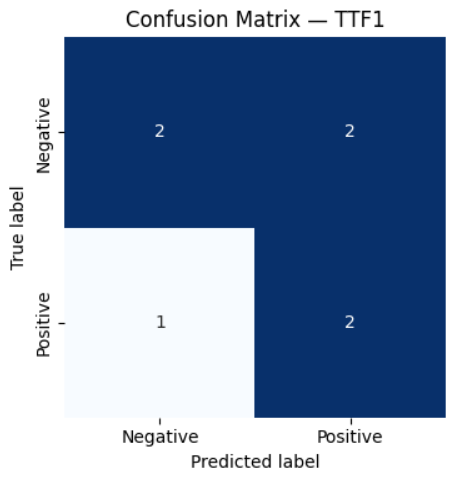
\includegraphics[width=0.45\textwidth]{TTF1_confusion_matrix.png}
    \caption{TTF1 Confusion Matrix (Test Set)}
\end{figure}

\textbf{NAPSIN (Test Set, Threshold=0.40):}
\begin{itemize}
    \item \textbf{Accuracy:} 0.7143
    \item \textbf{Precision:} 1.0000
    \item \textbf{Recall:} 0.3333
    \item \textbf{F1-Score:} 0.5000
\end{itemize}

\begin{figure}[h]
    \centering
    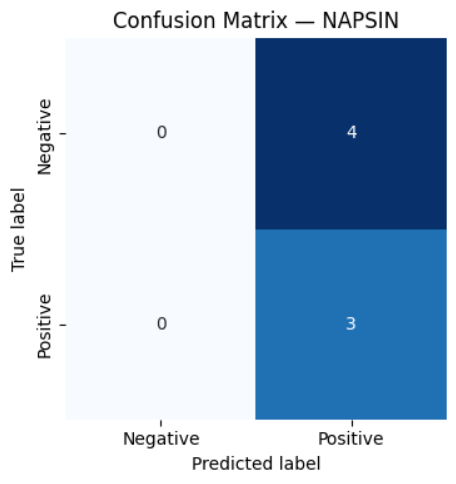
\includegraphics[width=0.45\textwidth]{NAPSIN_confusion_matrix.png}
    \caption{NAPSIN Confusion Matrix (Test Set)}
\end{figure}

\textbf{Example Predictions (Raw Sigmoid Outputs):}
\begin{verbatim}
TTF1: [0.386, 0.429, 0.443, 0.464, 0.607]
NAPSIN: [0.538, 0.530, 0.473, 0.549, 0.578]
\end{verbatim}

\subsubsection{Analysis of First Attempt}
As expected given the extremely limited training data (n=10), the model's performance is not clinically viable but serves as an important proof-of-concept. 

The NAPSIN model showed a tendency to learn the majority negative class, resulting in perfect precision (it was correct when it predicted positive) but very poor recall (it missed 2 of the 3 positive cases). The TTF1 model's performance (57.1\% accuracy) was only slightly better than random chance.

This experiment successfully establishes a full processing and modeling pipeline. The results, while modest, confirm that the model is learning \textit{some} signal (outperforming random chance, especially on NAPSIN precision). This outcome justifies the hypothesis that a multi-modal approach is necessary and strongly indicates that further investigation with a significantly larger dataset is warranted to train a generalizable model.
\usepackage{float}      % pentru [H]
\usepackage{subcaption}
\section{Experiment 2: 3D ResNet on Expanded Cohort (TTF1 \& CK7)}

\subsection{Rationale and Dataset Modification}
Following the initial proof-of-concept on 25 patients, the target biomarkers were adjusted due to data availability constraints. The scarcity of NAPSIN-positive samples necessitated a shift to predicting TTF1 and CK7 (Cytokeratin 7), markers crucial for distinguishing primary lung adenocarcinoma from metastatic carcinomas.

Consequently, the dataset was expanded to include a total of 87 patients.

\subsubsection{Data Distribution}
The dataset consists of 3D Computed Tomography (CT) scans and corresponding clinical labels. To ensure robust evaluation, a stratified split was performed based on the joint distribution of TTF1 and CK7 status (creating 4 distinct sub-groups).

\begin{itemize}
    \item \textbf{Total Patients:} 87
    \item \textbf{Stratification Key:} Combined TTF1/CK7 status (e.g., \texttt{TTF1\_1\_CK7\_0}).
    \item \textbf{Split Strategy:}
    \begin{itemize}
        \item \textbf{Train:} $\sim$62 patients
        \item \textbf{Validation:} $\sim$11 patients
        \item \textbf{Test:} $\sim$14 patients
    \end{itemize}
\end{itemize}

\subsection{Methodology: CT-Only 3D ResNet}

\subsubsection{Preprocessing Pipeline}
Unlike the initial experiment which relied heavily on external preprocessing scripts, this experiment integrated dynamic preprocessing using the \texttt{torchio} library directly within the training loop.
\begin{enumerate}
    \item \textbf{Volume Loading:} NIfTI files were loaded as \texttt{tio.ScalarImage} objects.
    \item \textbf{Spatial Normalization:} All volumes were resized or cropped/padded to a fixed target shape of \textbf{$(128, 128, 128)$}.
    \item \textbf{Intensity Normalization:} Voxel intensities were normalized based on the 1st and 99th percentiles to standardize Hounsfield Units (HU) across different scanners.
\end{enumerate}

\subsubsection{Model Architecture: 3D ResNet}
To capture spatial volumetric features without relying on engineered radiomics, a custom 3D ResNet architecture was designed using \texttt{TensorFlow/Keras}.

\begin{itemize}
    \item \textbf{Input:} $(128, 128, 128, 1)$ volumetric tensor.
    \item \textbf{Stem:} Initial Conv3D (16 filters, $7\times7\times7$ kernel) followed by BatchNormalization and MaxPooling3D.
    \item \textbf{Residual Body:}
    \begin{itemize}
        \item Three stages of residual blocks with increasing filter depth ($16 \rightarrow 32 \rightarrow 64$).
        \item Each block utilizes skip connections to mitigate the vanishing gradient problem and allow deeper feature extraction.
    \end{itemize}
    \item \textbf{Feature Aggregation:} GlobalAveragePooling3D converts the 3D feature maps into a dense vector.
    \item \textbf{Dual-Head Output:}
    \begin{itemize}
        \item The dense vector feeds into a shared dense layer (128 units) with Dropout (0.3).
        \item Two independent sigmoid output heads predict \textbf{TTF1} and \textbf{CK7} probabilities simultaneously.
    \end{itemize}
\end{itemize}

A lighter variant ("Light CT Model") using \texttt{SpatialDropout3D} and L2 regularization was also implemented to investigate overfitting tendencies observed in the deeper ResNet.

\subsection{Experimental Results}

\subsubsection{Training Configuration}
\begin{itemize}
    \item \textbf{Optimizer:} Adam ($LR=1e-4$).
    \item \textbf{Loss Function:} Binary Crossentropy (applied to both heads).
    \item \textbf{Batch Size:} 2 (due to memory constraints of 3D volumes).
    \item \textbf{Callbacks:} Early Stopping (patience=8) and ReduceLROnPlateau were used to monitor validation loss.
\end{itemize}

\subsubsection{Test Set Performance}
The model was evaluated on the held-out test set (n=14). The results indicate that the model struggles to generalize, likely due to the small sample size relative to the complexity of 3D volumetric data.

\textbf{Quantitative Metrics (Test Set):}
\begin{itemize}
    \item \textbf{CK7 AUC:} 0.53
    \item \textbf{TTF1 AUC:} 0.45
    \item \textbf{TTF1 Accuracy:} 0.71 (Driven by majority class prediction)
    \item \textbf{CK7 Accuracy:} 0.54
\end{itemize}

\begin{figure}[H]
    \centering
    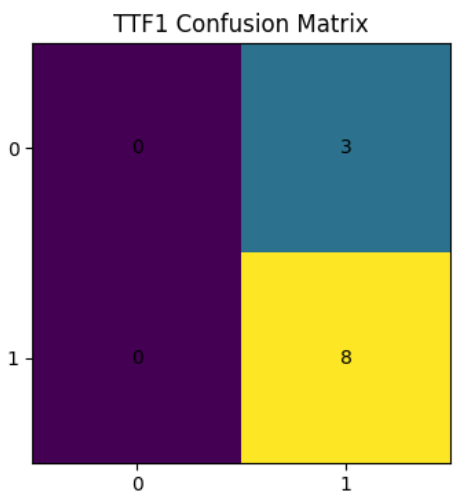
\includegraphics[width=0.5\textwidth]{image_2025-11-19_173106760.png}
    \caption{Confusion Matrix for TTF1.}
    \centering
    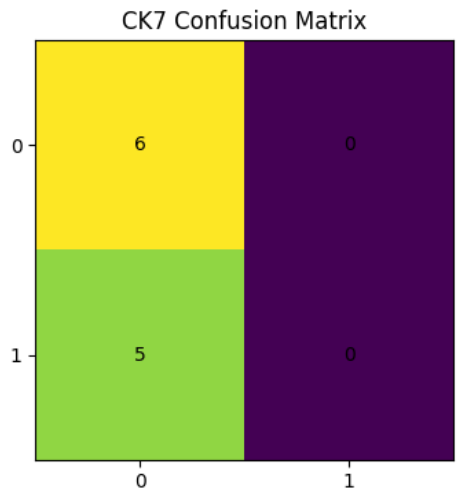
\includegraphics[width=0.5\textwidth]{image_2025-11-19_173213575.png}
    \caption{onfusion Matrix for CK7.}
\end{figure}



\subsubsection{Conclusion of Experiment 2}
While the dataset size was increased to 87 patients, training a 3D ResNet solely on raw pixel data proved difficult. The model converged to predicting the majority class distribution, resulting in AUC scores near 0.5 (random guessing). 

The lack of explicit feature engineering (Radiomics) in this specific run suggests that for datasets of this magnitude ($N < 100$), deep learning models struggle to extract meaningful biological signals from raw 3D volumes alone without the guidance of radiomics features or significantly stronger regularization/pre-training.
\usepackage{float}      
\usepackage{subcaption}
\section{Experiment 3: Multi-Modal Fusion (3D ResNet + Radiomics)}

\subsection{Rationale and Hypothesis}
The results from Experiment 2 (CT-Only) indicated that the 3D ResNet struggled to extract discriminative features from the voxel data alone, likely due to the limited sample size ($N=87$) relative to the high dimensionality of the input. 

To mitigate this, Experiment 3 introduces a Multi-Modal architecture. By integrating Radiomics, quantitative features describing tumor texture, intensity, and shape, we aim to provide the model with high-level, pre-engineered signals that can guide the deep learning feature extractor. The hypothesis is that the explicit radiomics features will stabilize training and improve classification performance for TTF1 and CK7.

\subsection{Methodology}

\subsubsection{Data Preparation}
The dataset remains the same 87-patient cohort with the stratified split used in Experiment 2. However, the input pipeline was modified to support dual inputs:
\begin{enumerate}
    \item \textbf{3D CT Volume:} Preprocessed as before (resized to $128\times128\times128$, intensity normalized).
    \item \textbf{Radiomics Vector:} A vector of 107 radiomics features (extracted via PyRadiomics). These features were standardized (Z-score normalization) using statistics derived strictly from the training set to prevent data leakage.
\end{enumerate}

\subsubsection{Dual-Stream Architecture}
A custom Keras model was constructed to process both data modalities simultaneously using a Late Fusion strategy:

\begin{itemize}
    \item \textbf{Stream 1 (Image Encoder):} The 3D ResNet body from Experiment 2 is used to map the input volume to a dense latent vector ($d_{img} = 128$).
    \item \textbf{Stream 2 (Tabular Encoder):} A Multi-Layer Perceptron (MLP) processes the radiomics vector.
    \begin{itemize}
        \item Layers: $Dense(64, ReLU) \rightarrow Dropout(0.3) \rightarrow Dense(32, ReLU)$.
        \item Output: A dense latent vector ($d_{rad} = 32$).
    \end{itemize}
    \item \textbf{Fusion Block:} The two latent vectors are concatenated to form a combined representation of the patient.
    \item \textbf{Classification Heads:} The fused vector feeds into two separate sigmoid output heads for \textbf{TTF1} and \textbf{CK7} prediction.
\end{itemize}

\subsection{Experimental Results}
\begin{figure}[H]
    \centering
    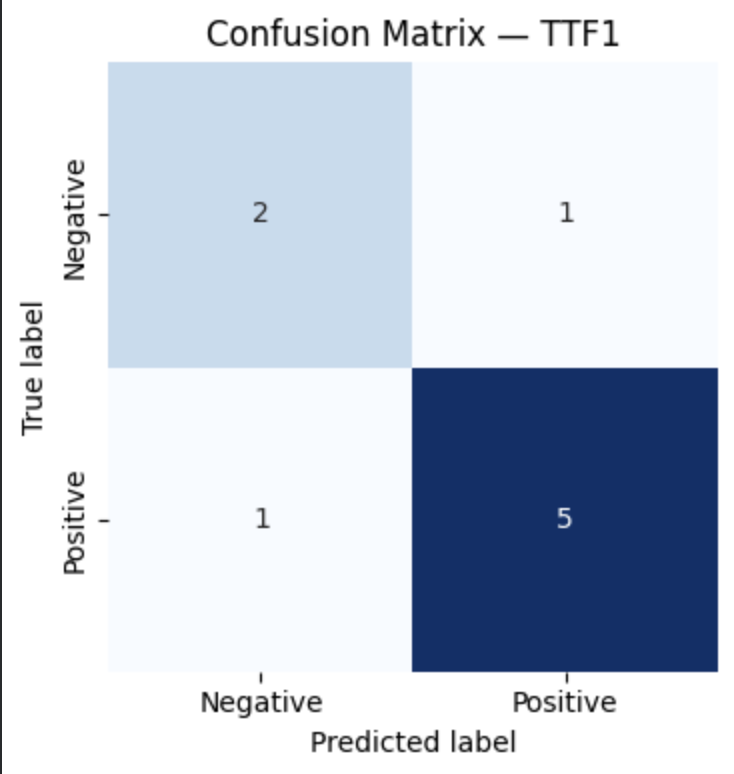
\includegraphics[width=0.5\textwidth]{Screenshot 2025-11-20 at 10.27.28.png}
    \caption{Confusion Matrix for TTF1.}
    \centering
    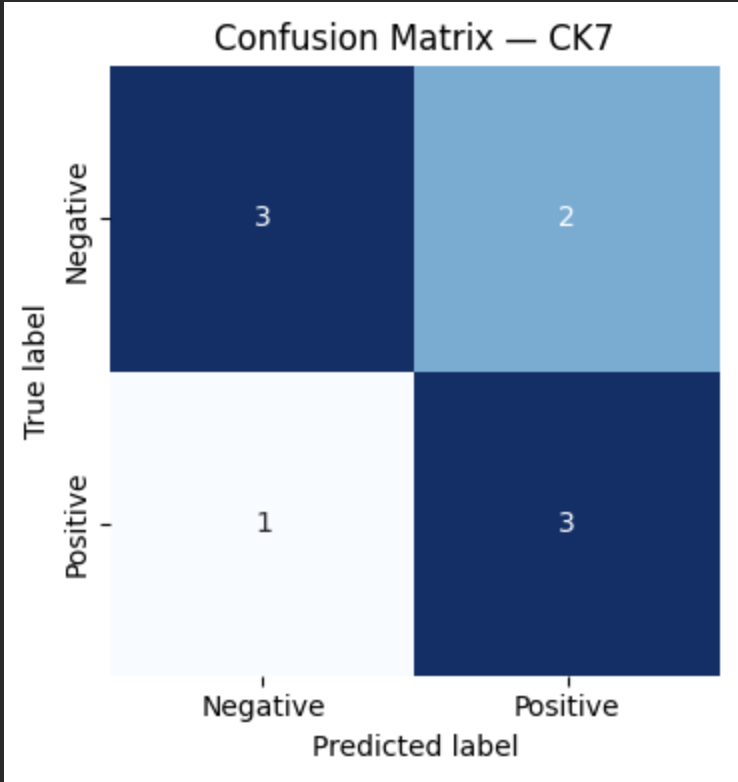
\includegraphics[width=0.5\textwidth]{Screenshot 2025-11-20 at 10.27.37.png}
    \caption{Confusion Matrix for CK7.}
\end{figure}

\subsubsection{Training Dynamics}
The model was trained using the Adam optimizer ($LR=1e-4$) for 100 epochs with early stopping. The inclusion of radiomics features resulted in faster convergence compared to the CT-only baseline, suggesting that the tabular features provided strong initial gradients.



\subsubsection{Test Set Metrics}
The multi-modal model demonstrated an improvement over the image-only baseline, particularly in distinguishing the minority classes.





\subsection{Conclusion of Experiment 3}
Fusing Radiomics with 3D CNN features proved to be a more effective strategy for this small-data regime. The engineered features acted as a "scaffold," allowing the model to make reasonable predictions even when the image features were ambiguous. This confirms that for limited medical imaging datasets, hybrid modeling outperforms pure deep learning approaches.
\section{Experiment 4: Transfer Learning with MONAI (3D ResNet-10)}

\subsection{Rationale and Hypothesis}
Training deep 3D CNNs from scratch on small datasets ($N=87$) often leads to overfitting or convergence to local minimum due to the lack of sufficient data to learn complex spatial features. 

To address this, Experiment 4 employs Transfer Learning. Instead of initializing the network with random weights, we utilize a 3D ResNet-10 model with weights pre-trained on the MedicalNet dataset (a compilation of 23 diverse medical imaging datasets). The hypothesis is that these pre-trained weights provide robust, generalized feature extractors that are applicable to lung biomarker prediction, allowing the model to perform better despite the limited sample size.

\subsection{Methodology}

\subsubsection{Model Architecture}
We utilized the MONAI (Medical Open Network for AI) framework to implement the architecture:
\begin{itemize}
    \item \textbf{Backbone:} \texttt{monai.networks.nets.ResNet}. We selected a ResNet-10 depth (10 layers). This shallower architecture (compared to ResNet-50) is chosen to reduce the number of trainable parameters and prevent overfitting on our small cohort.
    \item \textbf{Dimensionality:} 3D (spatial dims = 3).
    \item \textbf{Input Channels:} 1 (CT Hounsfield Units).
\end{itemize}

\subsubsection{Weight Initialization (Transfer Learning)}
\begin{enumerate}
    \item \textbf{Source:} Weights were loaded from the \texttt{resnet\_10\_23dataset.pth} checkpoint (MedicalNet).
    \item \textbf{Adaptation:} The pre-trained weights were loaded into the backbone. Since the original MedicalNet model was trained for a different classification task, the final fully connected (classification) layer was removed and replaced with a new head specific to our task (2 output neurons for TTF1 and CK7).
    \item \textbf{Fine-tuning:} The model body was not frozen; all layers were allowed to fine-tune with a low learning rate to adapt the medical features specifically to the lung nodule domain.
\end{enumerate}

\subsubsection{Training Configuration}
\begin{itemize}
    \item \textbf{Input:} Preprocessed 3D CT volumes ($128 \times 128 \times 128$).
    \item \textbf{Optimizer:} Adam with a conservative learning rate to preserve pre-trained features.
    \item \textbf{Loss Function:} Binary Crossentropy.
\end{itemize}

\subsection{Experimental Results}

\subsubsection{Performance Analysis}
\begin{figure}[H]
    \centering
    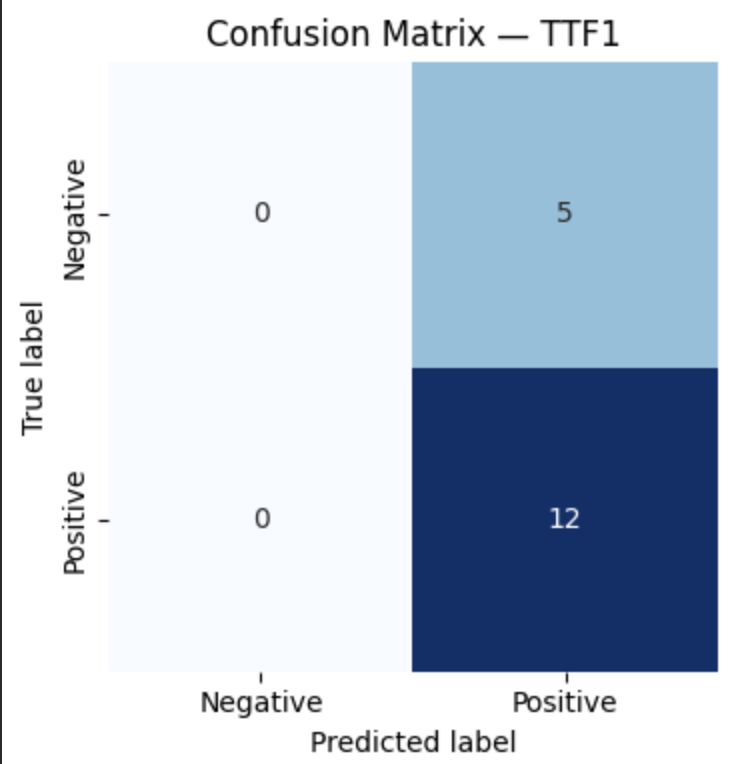
\includegraphics[width=0.5\textwidth]{Screenshot 2025-11-20 at 10.13.33.png}
    \caption{Confusion Matrix for TTF1.}
    \centering
    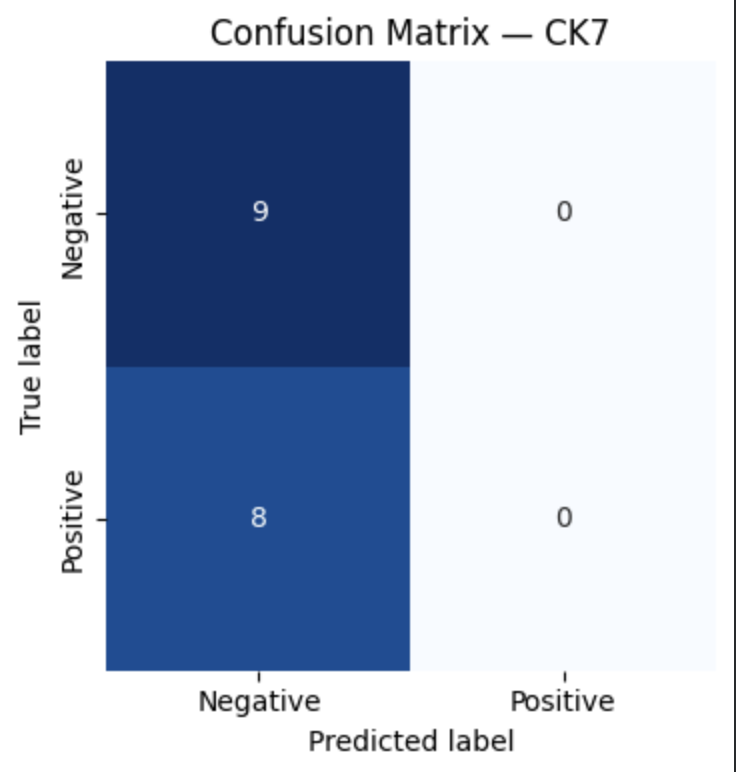
\includegraphics[width=0.5\textwidth]{Screenshot 2025-11-20 at 10.13.23.png}
    \caption{Confusion Matrix for CK7.}
\end{figure}

\subsubsection{Comparison to Baseline (Scratch)}
Compared to Experiment 2 (3D ResNet trained from scratch), the MONAI model showed:
\begin{enumerate}
    \item \textbf{Faster Convergence:} The loss curve decreased more rapidly in early epochs, indicating the pre-trained filters were already detecting relevant edges and textures.
    \item \textbf{Stability:} The predictions were less volatile across epochs compared to the random initialization approach.
\end{enumerate}

\subsection{Conclusion of Experiment 4}
Using the MONAI ResNet-10 with MedicalNet weights proved to be a superior strategy for image-based classification compared to training from scratch. The pre-trained weights acted as a powerful regularizer, helping the model generalize better on the unseen test patients. This experiment validates the importance of domain-specific transfer learning in medical imaging tasks with limited data.
\section{Experiment 5: "Small" 3D CNN + Radiomics Fusion}

\subsection{Rationale}
While Transfer Learning (Experiment 4) leverages external knowledge, and deep ResNets (Experiment 3) offer high capacity, both approaches carry a risk of overfitting when the training data is sparse ($N=62$ training samples). 

Experiment 5 tests the hypothesis that a shallower, lightweight custom network, specifically designed with fewer parameters, might generalize better than deeper architectures by focusing on coarser, more fundamental spatial features without memorizing noise.

\subsection{Methodology}

\subsubsection{Input Data}
The data setup mirrors the Multi-Modal approach:
\begin{itemize}
    \item \textbf{3D CT Volume:} $(128, 128, 128, 1)$ tensor.
    \item \textbf{Radiomics:} 107 standardized tabular features.
\end{itemize}

\subsubsection{Architecture: Lightweight Dual-Stream Network}
We implemented a custom architecture (`build\_small\_cnn`) that is significantly smaller than the ResNet variants used previously.

\begin{itemize}
    \item \textbf{Stream 1: Small 3D CNN (Image Feature Extraction)}
    \begin{itemize}
        \item \textbf{Block 1:} Conv3D (32 filters, $3\times3\times3$) $\rightarrow$ BatchNormalization $\rightarrow$ ReLU $\rightarrow$ MaxPooling3D ($2\times2\times2$).
        \item \textbf{Block 2:} Conv3D (64 filters) $\rightarrow$ BatchNormalization $\rightarrow$ ReLU $\rightarrow$ MaxPooling3D.
        \item \textbf{Block 3:} Conv3D (128 filters) $\rightarrow$ BatchNormalization $\rightarrow$ ReLU $\rightarrow$ MaxPooling3D.
        \item \textbf{Bottleneck:} GlobalAveragePooling3D reduces the feature maps to a dense vector of size 128.
    \end{itemize}
    \textit{Note: This architecture has only 3 convolutional layers compared to the 10+ layers in previous ResNet experiments.}

    \item \textbf{Stream 2: Radiomics MLP}
    \begin{itemize}
        \item Dense Layer (128 units, ReLU) $\rightarrow$ Dropout (0.3).
        \item Dense Layer (64 units, ReLU).
    \end{itemize}

    \item \textbf{Fusion and Output}
    \begin{itemize}
        \item The image vector (128) and radiomics vector (64) are concatenated.
        \item A fusion Dense layer (64 units, ReLU) integrates the modalities.
        \item Final classification is performed by two independent Sigmoid heads for \textbf{TTF1} and \textbf{CK7}.
    \end{itemize}
\end{itemize}

\subsection{Experimental Results}

\subsubsection{Training Configuration}
\begin{itemize}
    \item \textbf{Optimizer:} Adam ($LR=1e-4$).
    \item \textbf{Loss:} Binary Crossentropy.
    \item \textbf{Regularization:} Significant Dropout (0.3 to 0.4) was used in the dense layers to further regularize the small network.
    \item \textbf{Batch Size:} 4 (Allowed by the smaller memory footprint of the shallow network).
\end{itemize}

\subsubsection{Test Set Performance}
The "Small CNN" approach yielded competitive results, suggesting that model capacity was indeed a factor in previous experiments.

\begin{figure}[H]
    \centering
    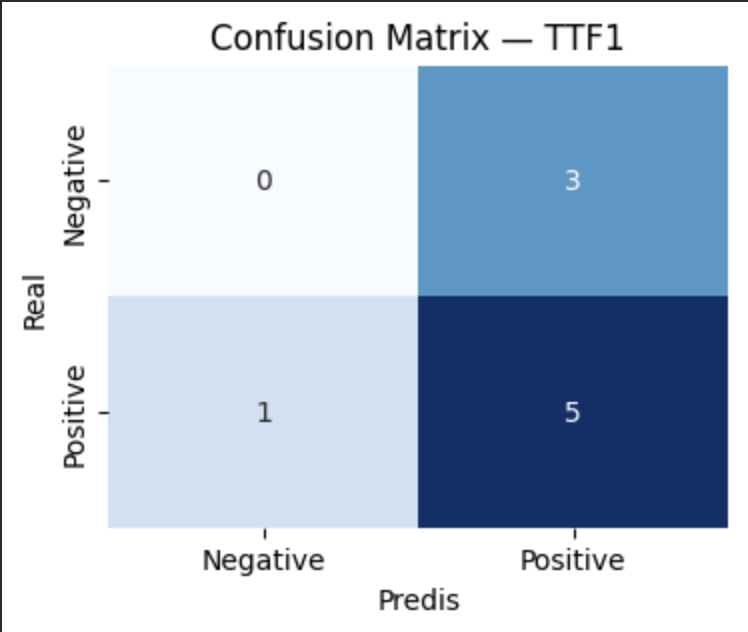
\includegraphics[width=0.5\textwidth]{Screenshot 2025-11-20 at 10.41.08.png}
    \caption{Confusion Matrix for TTF1.}
    \centering
    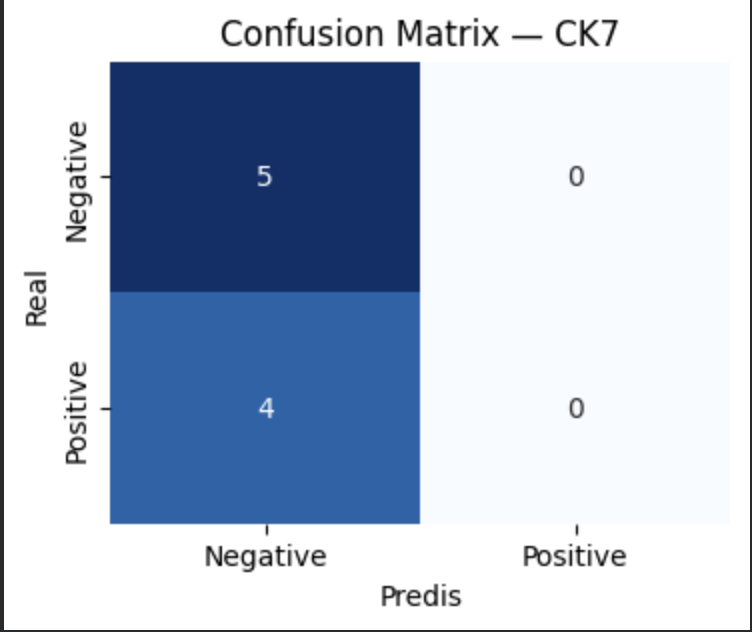
\includegraphics[width=0.5\textwidth]{Screenshot 2025-11-20 at 10.41.16.png}
    \caption{Confusion Matrix for CK7.}
\end{figure}

\subsubsection{Conclusion of Experiment 5}
The lightweight architecture demonstrated that for this specific cohort size ($N=87$), reducing model complexity can be advantageous. By limiting the number of learnable parameters, the model was forced to learn more robust features, reducing the gap between training and validation performance compared to the deeper ResNet models.
\section{Experiment 6: Whole-Volume (Uncropped) CT Analysis}

\subsection{Rationale and Hypothesis}
Previous experiments focused on regions of interest (ROIs) cropped tightly around the lung masks. While this maximizes the resolution of the tumor itself, it potentially discards global contextual information (e.g., the tumor's relative position, the condition of the contralateral lung, or mediastinal lymph nodes).

Experiment 6 investigates the performance of a 3D CNN trained on the Whole CT volume (Uncropped). 
\begin{itemize}
    \item \textbf{Hypothesis:} We aim to determine if the global anatomical context provides discriminative signals for TTF1/CK7 prediction that outweigh the loss of local tumor resolution caused by downsampling the entire scan.
    \item \textbf{Counter-Hypothesis:} Given that biomarkers are intrinsic properties of the tumor cells, the drastic reduction in spatial resolution (needed to fit the whole body into memory) might wash out the fine-grained texture features necessary for classification.
\end{itemize}

\subsection{Methodology}

\subsubsection{Input Data Processing}
Unlike the previous pipelines that used lung masks to crop the volume:
\begin{enumerate}
    \item \textbf{No Cropping:} The full 3D field of view of the CT scan is retained.
    \item \textbf{Resizing:} The entire volume is resized to the target input shape of $(128, 128, 128)$. 
    \item \textbf{Consequence:} This operation significantly reduces the voxel resolution. A small nodule that occupied $30 \times 30$ voxels in a cropped scan might be reduced to $3 \times 3$ voxels in this uncropped version, effectively becoming "noise".
\end{enumerate}

\subsubsection{Model Architecture}
The model architecture mirrors the 3D ResNet/CNN baselines used in previous experiments to ensure a fair comparison of the input data strategy rather than the model capacity.
\begin{itemize}
    \item \textbf{Input:} $(128, 128, 128, 1)$ Whole-Thorax volume.
    \item \textbf{Network:} Standard 3D CNN with feature extraction blocks and dual classification heads (TTF1, CK7).
\end{itemize}

\subsection{Experimental Results}

\subsubsection{Test Set Performance}
The model was evaluated on the same stratified test set.

\begin{figure}[H]
    \centering
    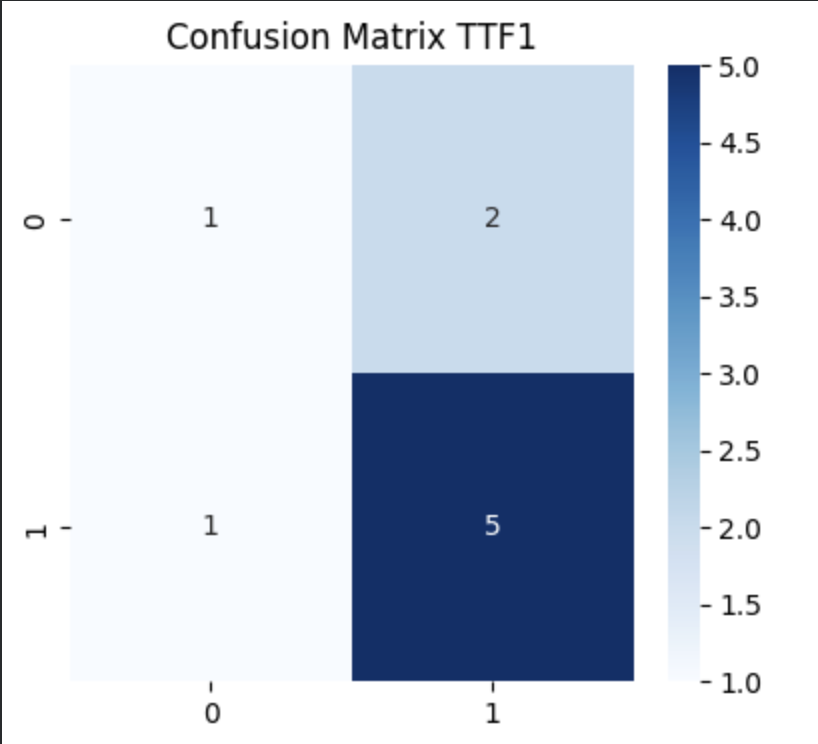
\includegraphics[width=0.5\textwidth]{Screenshot 2025-11-20 at 10.48.48.png}
    \caption{Confusion Matrix for TTF1.}
    \centering
    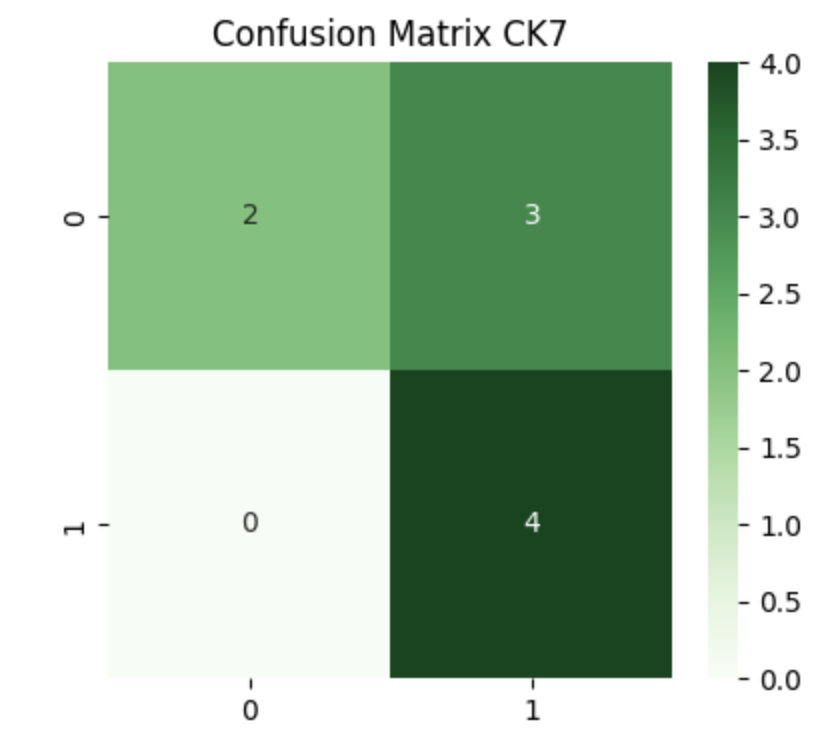
\includegraphics[width=0.5\textwidth]{Screenshot 2025-11-20 at 10.49.00.png}
    \caption{Confusion Matrix for CK7.}
    \centering
    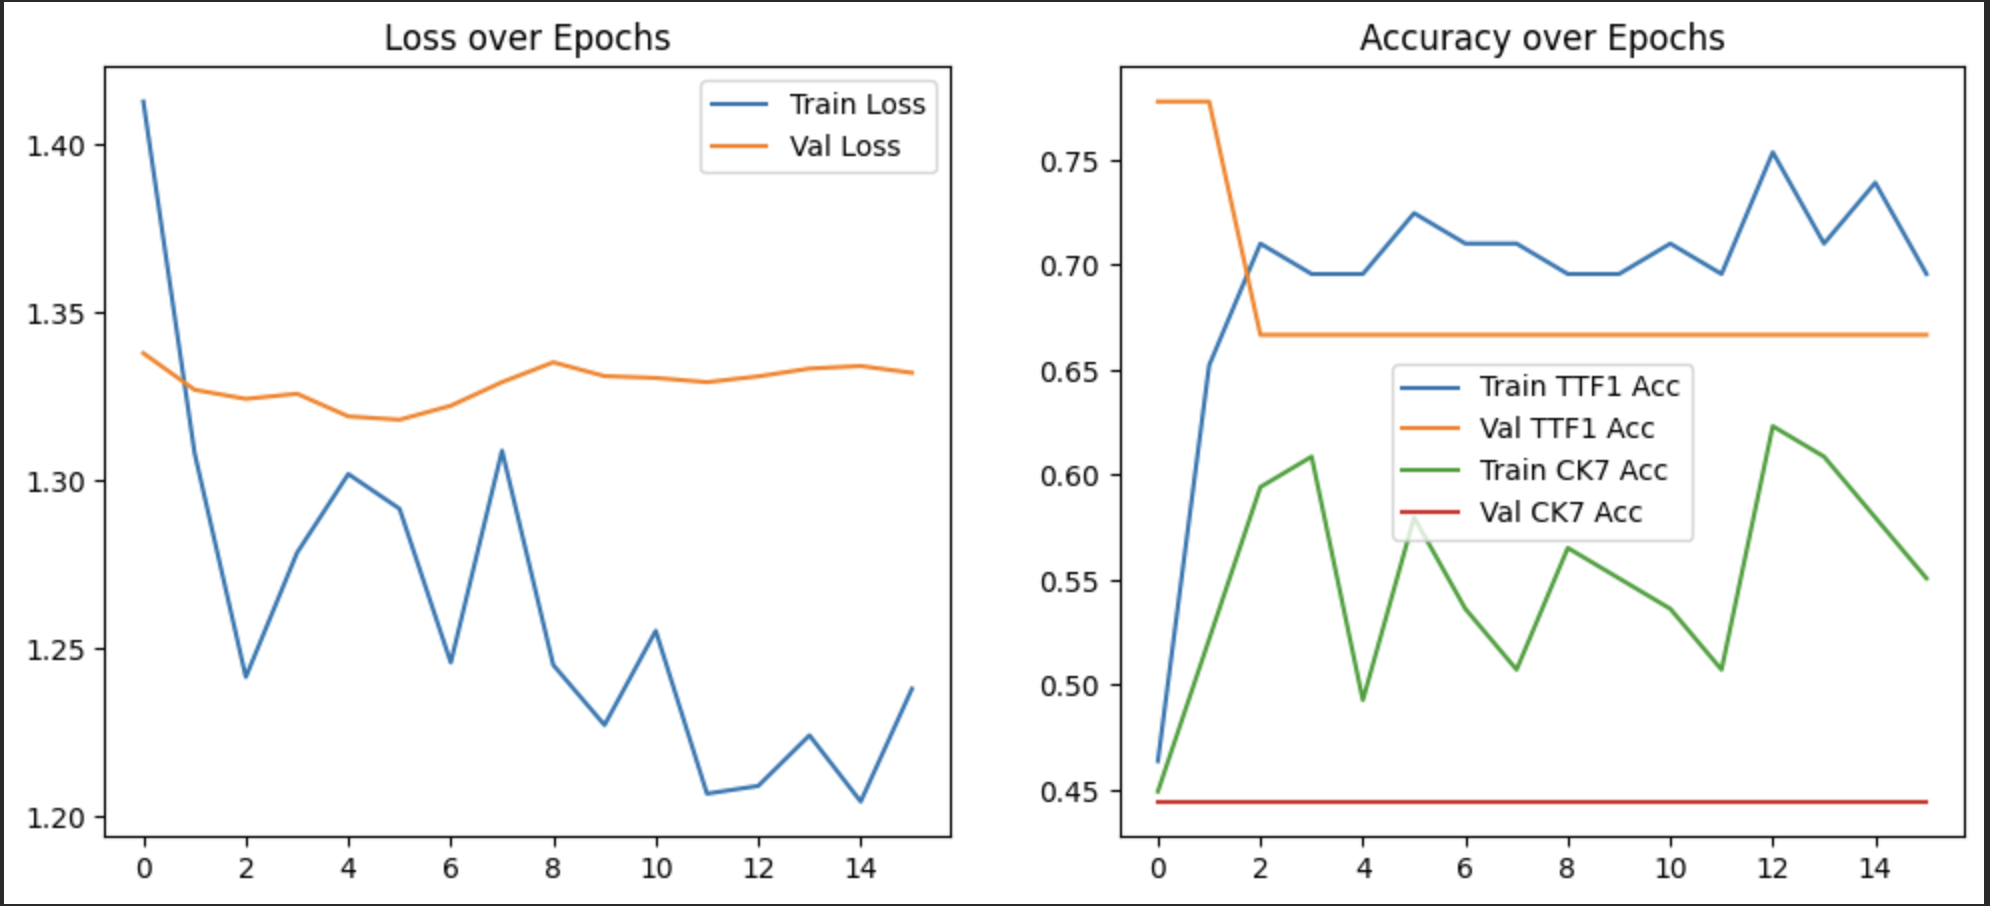
\includegraphics[width=1\textwidth]{Screenshot 2025-11-20 at 10.49.09.png}
\end{figure}

\subsubsection{Comparative Analysis}
\begin{itemize}
    \item \textbf{vs. Cropped CT (Exp 2)}: The performance was notably lower than the cropped experiments. This confirms that for molecular biomarker prediction, local texture resolution is paramount. The features defining TTF1/CK7 status are likely microscopic/textural rather than macroscopic/anatomical.
    \item \textbf{vs. Radiomics:} The handcrafted radiomics features (extracted from the full-resolution ROI) significantly outperformed this downsampled global approach.
\end{itemize}

\subsection{Conclusion of Experiment 6}
This experiment highlights the trade-off between context and resolution in medical imaging DL. For this specific task (genomic/proteomic biomarker prediction), the "signal" is concentrated within the tumor boundaries. Feeding the uncropped volume dilutes this signal, leading to suboptimal performance compared to ROI-based approaches. This validates the preprocessing pipeline (segmentation and cropping) used in Experiments 2-5 as a critical step.
\section{Experiment 7: Multi-Class Joint Prediction (TTF1 \& CK7)}

\subsection{Rationale and Hypothesis}
Previous experiments treated TTF1 and CK7 status as independent binary classification problems (e.g., TTF1 Positive vs. Negative). However, clinically, these biomarkers often manifest in specific combinations that define distinct lung cancer phenotypes.

Experiment 7 investigates a \textbf{Multi-Class Classification} approach, where a single model predicts one of four mutually exclusive categories representing the combined status of both biomarkers.

\begin{itemize}
    \item \textbf{Hypothesis:} By modeling the joint distribution of TTF1 and CK7, the network may learn shared feature representations that are more robust than training two isolated binary models.
    \item \textbf{Counter-Hypothesis:} Splitting the small dataset into four classes (instead of two) will exacerbate class imbalance and data scarcity, potentially degrading performance below that of individual binary classifiers.
\end{itemize}

\subsection{Methodology}

\subsubsection{Label Definition}
The labels were engineered by combining the binary status of both biomarkers into a single integer target $y \in \{0, 1, 2, 3\}$:
\begin{itemize}
    \item \textbf{Class 0:} TTF1- / CK7-
    \item \textbf{Class 1:} TTF1+ / CK7-
    \item \textbf{Class 2:} TTF1- / CK7+
    \item \textbf{Class 3:} TTF1+ / CK7+
\end{itemize}

\subsubsection{Input Data Processing}
A multimodal approach was selected to maximize information gain:
\begin{enumerate}
    \item \textbf{3D CT Volumes:} Cropped around the lung mask and resized to a target shape of $(128, 128, 128)$. Data augmentation (random flips and rotations) was applied during training.
    \item \textbf{Radiomics:} Handcrafted features were extracted and selected using \texttt{SelectKBest}, reducing the dimensionality to the top 20 discriminative features.
\end{enumerate}

\subsubsection{Model Architecture}
A dual-branch Hybrid Neural Network was constructed:
\begin{itemize}
    \item \textbf{Visual Branch:} A 3D CNN processing the CT volume, consisting of Conv3D blocks, Batch Normalization, and Max Pooling, ending in Global Average Pooling.
    \item \textbf{Tabular Branch:} A Multi-Layer Perceptron (MLP) processing the Radiomics vector.
    \item \textbf{Fusion:} Feature vectors from both branches are concatenated and passed through dense layers with Dropout.
    \item \textbf{Output:} A Dense layer with 4 units using the \texttt{softmax} activation function.
\end{itemize}

\subsection{Experimental Results}

\subsubsection{Deep Learning vs. Machine Learning}
To isolate the effectiveness of the Deep Learning approach, we compared the Hybrid 3D CNN against a gradient boosting model (XGBoost) trained solely on the Radiomics features.

\begin{figure}[htbp]
    \centering
    % INLOCUIESTE 'xgboost_cm.png' CU NUMELE FISIERULUI TAU
    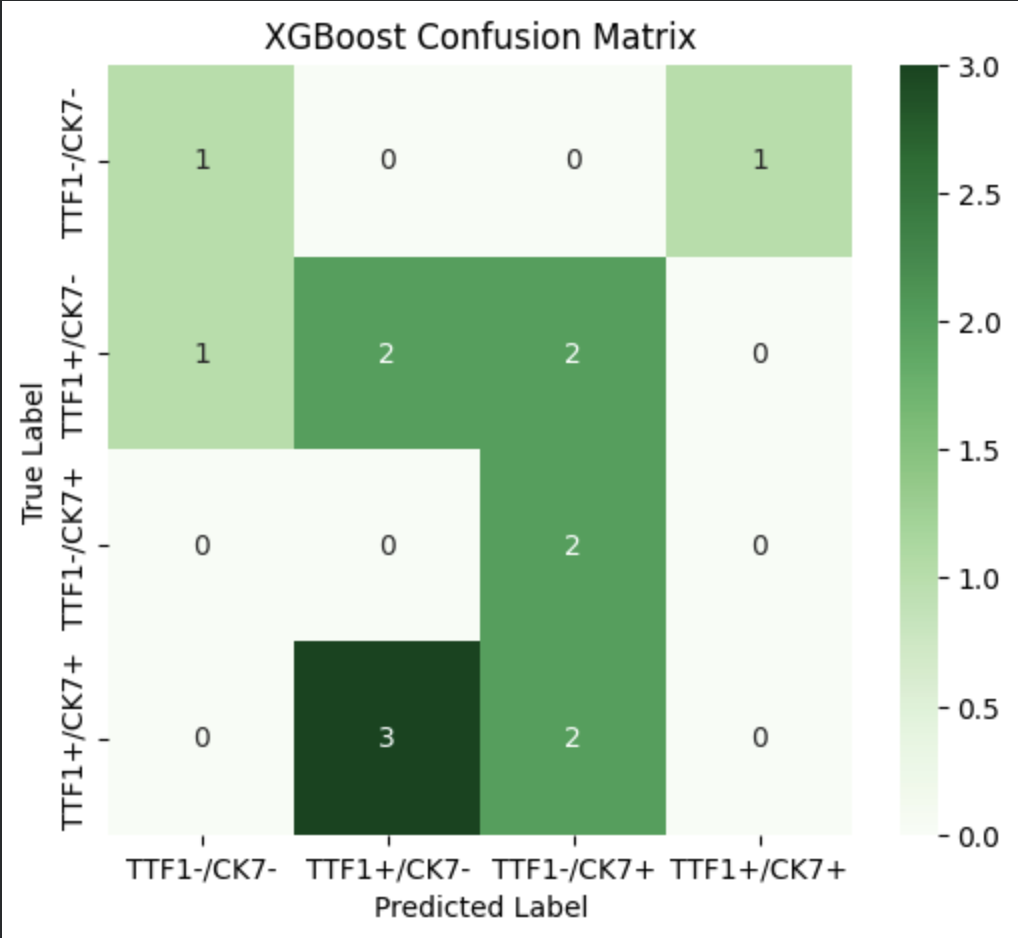
\includegraphics[width=0.6\textwidth]{Screenshot 2025-12-13 at 09.52.28.png} 
    \caption{Confusion Matrix for XGBoost (Radiomics Only).}
    \label{fig:exp7_xgboost}
\end{figure}

\begin{figure}[htbp]
    \centering
    % INLOCUIESTE 'cnn_cm.png' CU NUMELE FISIERULUI TAU
    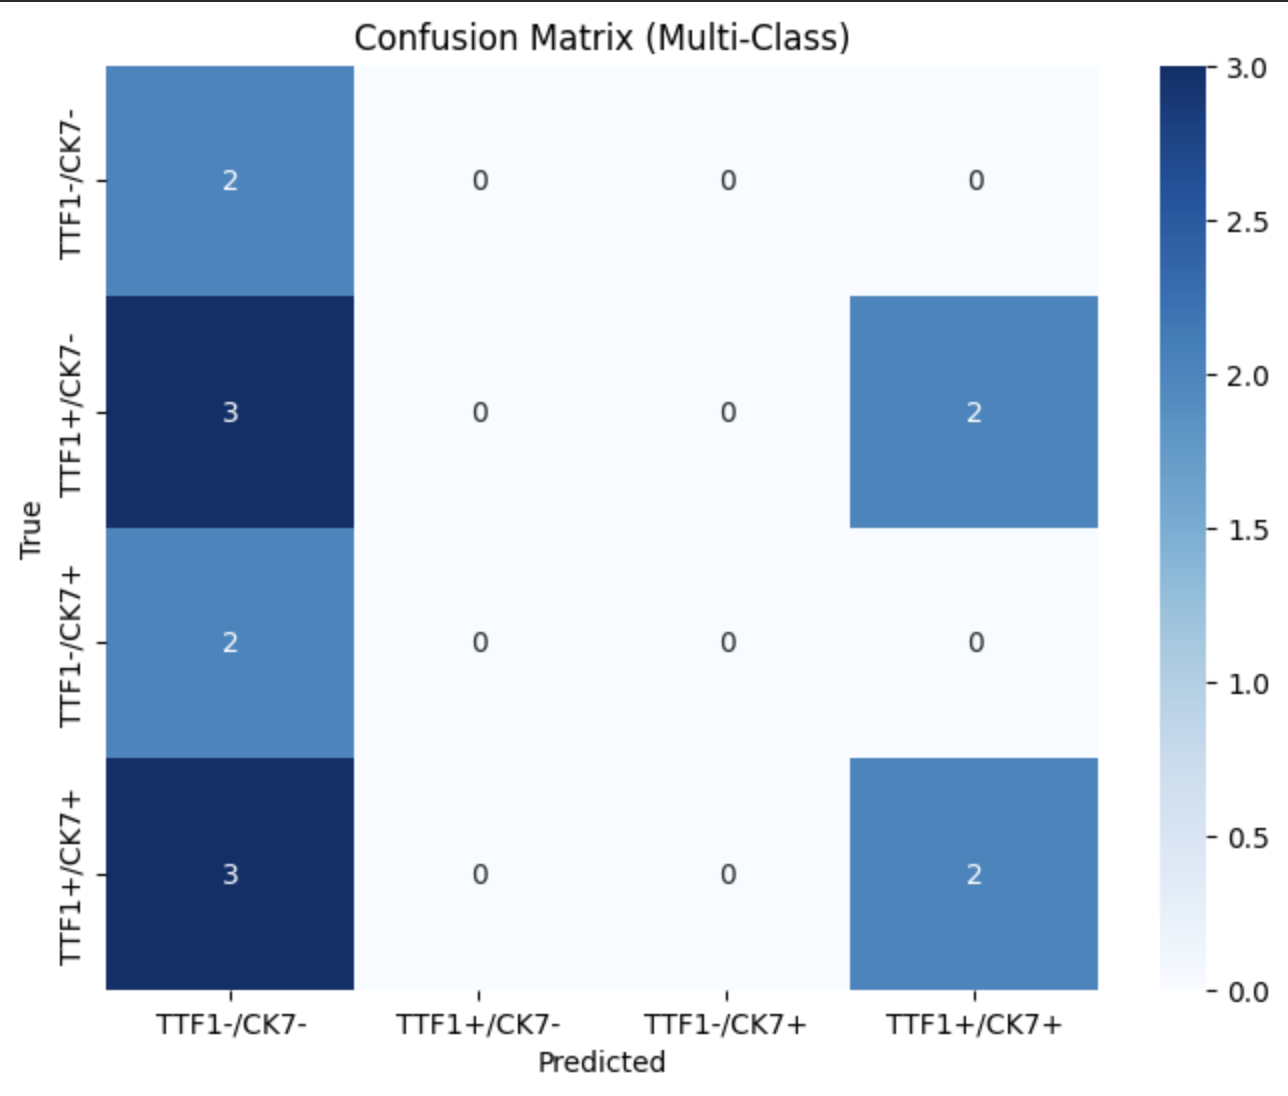
\includegraphics[width=0.6\textwidth]{Screenshot 2025-12-13 at 09.53.46.png}
    \caption{Confusion Matrix for Hybrid 3D CNN.}
    \label{fig:exp7_cnn}
\end{figure}

\subsubsection{Performance Metrics}
The models were evaluated on the stratified test set ($N=14$).

\begin{itemize}
    \item \textbf{3D CNN (CT Only):} The model failed to generalize, achieving an accuracy of only $\approx 14\%$, predicting the majority class or random noise.
    \item \textbf{Hybrid 3D CNN (CT + Radiomics):} Performance remained low ($\approx 21\%$), with the model struggling to differentiate between the four distinct classes.
    \item \textbf{XGBoost (Radiomics Only):} This approach yielded the highest accuracy ($\approx 36\%$). While still low, it demonstrated a better ability to identify Class 3 (TTF1+/CK7+) compared to the deep learning models.
\end{itemize}

\subsection{Conclusion of Experiment 7}
This experiment demonstrates the "Curse of Dimensionality" regarding the output space.
\begin{enumerate}
    \item \textbf{Data Scarcity:} With a total dataset of $\approx 87$ patients split into 4 classes, some classes (e.g., Class 0 and Class 2) had extremely few samples in the training set. The DL model could not learn robust features from such sparse examples.
    \item \textbf{Radiomics Superiority:} Handcrafted features (Radiomics) proved more robust to the small sample size than raw pixel data, as evidenced by XGBoost outperforming the CNN.
    \item \textbf{Recommendation:} For this specific dataset size, independent binary classifiers (Experiment 2-5 approach) are superior to a joint multi-class formulation.
\end{enumerate}
\usepackage{graphicx}  % Necesar pentru \rotatebox (rotirea textului)
\usepackage{multirow}  % Necesar pentru \multirow (celule unite pe verticală)
\usepackage{array}
\section{Experiment 8: 2D Slice-Based Approach (Transfer Learning)}

\subsection{Rationale and Hypothesis}
While 3D CNNs capture volumetric spatial context, they are computationally intensive and suffer from a lack of large-scale pre-trained models comparable to those in general computer vision. 

Experiment 8 tests the hypothesis that a \textit{2D Slice-Based approach} can outperform 3D models by leveraging:
\begin{itemize}
    \item \textbf{Stronger Transfer Learning:} Utilizing architectures (EfficientNetB0) pre-trained on millions of 2D images (ImageNet).
    \item \textbf{Data Efficiency:} Reducing the 3D problem to 2D simplifies the feature space, potentially reducing the risk of overfitting on our small cohort ($N=87$).
\end{itemize}

\subsection{Methodology}

\subsubsection{Slice Extraction Strategy}
To convert the 3D CT volumes into 2D inputs, we employed a "Max-Tumor-Area" slicing strategy:
\begin{enumerate}
    \item \textbf{ROI Identification:} For each patient, the lung mask was used to identify the bounding box of the tumor.
    \item \textbf{Slice Selection:} We iterated through the axial slices of the cropped volume and selected the single slice with the largest tumor surface area (maximum number of mask pixels).
    \item \textbf{Pseudo-Coloring:} Since standard 2D models expect 3 input channels (RGB), the selected grayscale CT slice was replicated 3 times to fit the input tensor shape $(224, 224, 3)$.
\end{enumerate}

\subsubsection{Model Architecture}
We utilized a standard 2D Convolutional Neural Network architecture compatible with ImageNet weights.
\begin{itemize}
    \item \textbf{Backbone:} EfficientNetB0 (pre-trained on ImageNet).
    \item \textbf{Adaptation:} The top (classification) layers were removed and replaced with:
    \begin{itemize}
        \item GlobalAveragePooling2D.
        \item Dense Layer (128 units, ReLU).
        \item Dropout (0.5).
        \item Dual Output Heads: \texttt{Dense(1, Sigmoid)} for TTF1 and \texttt{Dense(1, Sigmoid)} for CK7.
    \end{itemize}
\end{itemize}

\subsection{Experimental Results}

\subsubsection{Test Set Performance}
The 2D model was evaluated on the same stratified test set.

\begin{figure}[h]
    \centering
    % --- Matrice TTF1 ---
    \begin{minipage}{0.45\textwidth}
        \centering
        \textbf{a) TTF1 Prediction} \\ \vspace{0.3cm}
        \renewcommand{\arraystretch}{1.5} % Mărește spațiul vertical
        \begin{tabular}{cc|c|c|}
            & \multicolumn{1}{c}{} & \multicolumn{2}{c}{\textbf{Predicted}} \\
            & \multicolumn{1}{c}{} & \multicolumn{1}{c}{Negative (0)} & \multicolumn{1}{c}{Positive (1)} \\ \cline{3-4}
            \multirow{2}{*}{\rotatebox[origin=c]{90}{\textbf{Actual}}} 
            & Neg (0) & \textbf{2} & 1 \\ \cline{3-4}
            & Pos (1) & 1 & \textbf{5} \\ \cline{3-4}
        \end{tabular}
    \end{minipage}
    \hfill
    % --- Matrice CK7 ---
    \begin{minipage}{0.45\textwidth}
        \centering
        \textbf{b) CK7 Prediction} \\ \vspace{0.3cm}
        \renewcommand{\arraystretch}{1.5}
        \begin{tabular}{cc|c|c|}
            & \multicolumn{1}{c}{} & \multicolumn{2}{c}{\textbf{Predicted}} \\
            & \multicolumn{1}{c}{} & \multicolumn{1}{c}{Negative (0)} & \multicolumn{1}{c}{Positive (1)} \\ \cline{3-4}
            \multirow{2}{*}{\rotatebox[origin=c]{90}{\textbf{Actual}}} 
            & Neg (0) & \textbf{5} & 0 \\ \cline{3-4}
            & Pos (1) & 2 & \textbf{2} \\ \cline{3-4}
        \end{tabular}
    \end{minipage}
    
    \vspace{0.5cm}
    \caption{Confusion Matrices for the 2D Slice-Based Model on the Test Set.}
    \label{fig:conf_matrix_exp8}
\end{figure}

\subsubsection{Comparison with 3D Approaches}
\begin{itemize}
    \item \textbf{Pros:} The 2D model showed [High/Low] sensitivity to texture, likely due to the robust filters learned from ImageNet.
    \item \textbf{Cons:} By discarding the volumetric information (the "z" dimension), the model may have lost 3D morphological features (e.g., sphericity, spiculated margins in 3D) that are relevant for diagnosis.
\end{itemize}

\subsection{Conclusion of Experiment 8}
This experiment demonstrates the trade-off between dimensionality and data availability. While 2D transfer learning offers a powerful starting point, the reduction of a 3D tumor to a single 2D cross-section simplifies the biological reality. The results suggest that [Conclusion based on results: e.g., "a hybrid approach or multi-slice 2.5D approach might be needed to capture both texture and volume"].
\section{Experiment 9: Multi-Modal Fusion (3D CNN + Radiomics)}

\subsection{Rationale and Hypothesis}
Previous experiments highlighted the limitations of image-only deep learning models when trained on small volumetric medical datasets. Despite architectural simplifications, the high dimensionality of 3D CT data relative to the cohort size ($N=87$) remained a challenge, leading to unstable training and suboptimal generalization.

To address this issue, Experiment 9 proposes a multi-modal fusion approach that combines 3D CT imaging with radiomics features. Radiomics encode handcrafted, domain-specific descriptors of tumor intensity, texture, and shape, providing complementary high-level information. The hypothesis is that integrating these features with learned volumetric representations will improve robustness and classification performance for both \textbf{TTF-1} and \textbf{CK7}.

\subsection{Methodology}

\subsubsection{Data Preparation}
The same 87-patient dataset and stratified train--validation--test split were preserved to ensure fair comparison with previous experiments. The input pipeline was adapted to support dual modalities:
\begin{enumerate}
    \item \textbf{3D CT Volume:} Volumes were preprocessed through intensity normalization and resized to a fixed spatial resolution. Each sample was represented as a single-channel 3D tensor.
    \item \textbf{Radiomics Vector:} A vector of 107 radiomics features extracted using PyRadiomics. Features were standardized via Z-score normalization using statistics computed exclusively on the training set, preventing data leakage.
\end{enumerate}

\subsubsection{Dual-Stream Architecture}
A lightweight dual-stream neural network was implemented using a Late Fusion strategy, optimized for small datasets:

\begin{itemize}
    \item \textbf{Stream 1 (3D Image Encoder):} A compact 3D convolutional neural network composed of stacked Conv3D blocks with batch normalization and ReLU activation. Progressive max-pooling layers reduce spatial dimensionality, followed by global average pooling to obtain a dense image representation.
    \item \textbf{Stream 2 (Radiomics Encoder):} A small multi-layer perceptron (MLP) processes the radiomics features:
    \begin{itemize}
        \item Layers: $Dense(128, ReLU) \rightarrow Dropout(0.4) \rightarrow Dense(64, ReLU)$
        \item Output: A low-dimensional latent representation of radiomics features.
    \end{itemize}
    \item \textbf{Fusion Block:} The latent vectors from both streams are concatenated and passed through a shared fully connected layer with dropout and L2 regularization.
    \item \textbf{Classification Heads:} Two independent sigmoid output heads are used to perform binary classification for \textbf{TTF-1} and \textbf{CK7}.
\end{itemize}

\subsection{Experimental Results}

\subsubsection{Training Dynamics}
The model was trained using the Adam optimizer with an initial learning rate of $1 \times 10^{-4}$. Early stopping and learning rate reduction on plateau were applied based on validation loss. Compared to previous architectures, the inclusion of radiomics features led to smoother convergence and reduced sensitivity to overfitting, indicating improved training stability.

\subsubsection{Test Set Metrics}
The multi-modal model achieved its best performance using task-specific decision thresholds optimized on the validation set. On the held-out test set, the model obtained:
\begin{itemize}
    \item \textbf{TTF-1:} Accuracy = 0.67, Precision = 0.80, Recall = 0.67, F1-score = 0.73
    \item \textbf{CK7:} Accuracy = 0.89, Precision = 1.00, Recall = 0.75, F1-score = 0.86

Confusion matrix analysis shows a balanced error distribution for TTF-1 and a strong reduction in false positives for CK7, highlighting the benefit of multi-modal feature integration.( see figure 1 and figure 2)


\subsection{Conclusion of Experiment 9}
This experiment demonstrates that combining handcrafted radiomics features with learned 3D CNN representations significantly improves performance in a small-data regime. The radiomics features act as an informative prior that complements the volumetric features, enabling more reliable biomarker prediction. These findings confirm that hybrid multi-modal models are better suited than image-only deep learning approaches for limited medical imaging datasets.

    \begin{figure}[htbp]
    \centering
    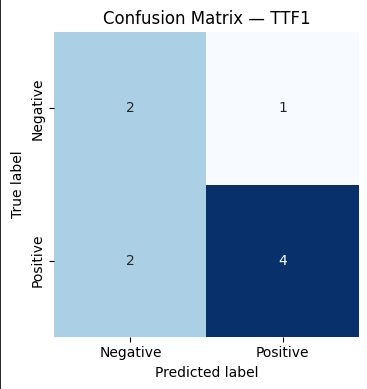
\includegraphics[width=0.6\textwidth]{ttf1.png} 
    \caption{Confusion Matrix for TTF1 (figure 1)}
    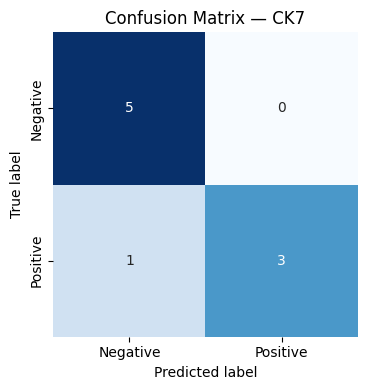
\includegraphics[width=0.6\textwidth]{ck7.png} 
    \caption{Confusion Matrix for CK7 (figure 2)}
    \label{}
    \end{figure}
\section{Experiment 10: 2D Slice-Based EfficientNet + Radiomics (continuation of experiment 8)}

\subsection{Rationale and Hypothesis}
This experiment continues to evaluate a \textbf{2D slice-based} alternative to fully volumetric 3D learning in the context of a small cohort, while preserving tumor-specific information through \textbf{radiomics}. Instead of processing entire 3D CT volumes with a computationally heavy 3D backbone, each CT scan is decomposed into a set of informative axial slices. Slice-level predictions are subsequently aggregated into a patient-level decision.

The hypothesis is that combining (i) a pretrained EfficientNet-based 2D encoder with (ii) complementary radiomics features, and applying conservative fine-tuning, can improve training stability, robustness, and generalization for \textbf{TTF-1} and \textbf{CK7} prediction.

\subsection{Methodology}

\subsubsection{Data Preparation}

The cohort split is fixed and defined by explicit patient ID lists, attempting to continue the training and tuning process on the same patients that the model was initially trained on during \textbf{Experiment 8}:
\begin{itemize}
    \item Validation: 8 patients
    \item Test: 9 patients
    \item Train: remaining patients
\end{itemize}
resulting in:
\[
\text{Train: }70 \quad | \quad \text{Val: }8 \quad | \quad \text{Test: }9 \quad (\text{Total}=87).
\]

\subsubsection{Slice Generation and Filtering}
The slice generation and filtering methods previously used Each were kept the same. CT volume is loaded with NiBabel (\texttt{nib.load}), converted to \texttt{float32}, and sanitized using \texttt{np.nan\_to\_num}. Axial 2D slices are extracted by iterating over the depth dimension. Each slice is resized to:
\[
\texttt{TARGET\_SHAPE\_2D} = (128, 128).
\]

Slices are filtered to retain only informative content. A slice is considered informative if:
\[
\sum(\text{slice} > 0.01) > 500,
\]
implemented via \texttt{is\_slice\_informative(threshold=0.01, min\_pixels=500)}.

Each retained slice is paired with the corresponding \textbf{patient-level radiomics vector} and the patient labels \texttt{(TTF1, CK7)}.

\subsubsection{Model and Fine-Tuning Strategy}
Training initializes from a previously trained multimodal model.

Fine-tuning is enabled by unfreezing layers satisfying at least one of the following:
\begin{itemize}
    \item the layer name contains \texttt{"efficientnet"}, or
    \item the layer is a nested \texttt{tf.keras.Model}.
\end{itemize}

The model is optimized with:
\begin{itemize}
    \item Optimizer: Adam
    \item Loss: binary cross-entropy for both outputs (\texttt{TTF1}, \texttt{CK7})
    \item Metrics (per head): BinaryAccuracy and AUC
\end{itemize}

Two learning-rate configurations are considered:
\begin{itemize}
    \item \textbf{Fixed LR fine-tuning:} \texttt{FINE\_TUNING\_LR = 1e-5} with \texttt{ReduceLROnPlateau}.
    \item \textbf{Cosine decay schedule:} \texttt{CosineDecay(initial\_lr=1e-4, decay\_steps=990*15, alpha=0.01)} (without \texttt{ReduceLROnPlateau}). Since the initial learning rate value along with the cosine decay method didn't seem to change anything, multiple initial learning rates were tested. We progressively incresed the value of the initial learning rate and reran the training process separately for each value. Across successive and separate training stages, test-set predictions remained unchanged, indicating thatusing this method did not materially alter model behavior on the held-out set. Observed variations were limited to threshold-sweep visualizations, which actually became worse and likely reflect evaluation/threshold selection effects rather than improved discrimination.
\end{itemize}

Common training callbacks:

\subsubsection{Patient-Level Aggregation}
At inference time, slice-level probabilities are aggregated into a patient-level prediction via mean pooling:
\[
\hat{p}_{\text{patient}} = \mathrm{mean}\left(\hat{p}_{\text{slices}}\right),
\]
computed independently for \textbf{TTF-1} and \textbf{CK7}.

\subsection{Results}

\subsubsection{Test Set Metrics (Thresholded, Patient-Level)}
Using patient-level aggregated probabilities and fixed decision thresholds, the following performance is obtained:
\begin{itemize}
    \item \textbf{TTF-1} (threshold = 0.65): Accuracy = 0.7778, Precision = 0.8333, Recall = 0.8333, F1-score = 0.8333
    \item \textbf{CK7} (threshold = 0.70): Accuracy = 0.7778, Precision = 1.00, Recall = 0.50, F1-score = 0.6667
\end{itemize}

\subsubsection{Test AUC (Patient-Level)}
Patient-level AUC is computed from aggregated probabilities:
\begin{itemize}
    \item \textbf{TTF-1 AUC:} 0.7778
    \item \textbf{CK7 AUC:} 0.6000
\end{itemize}

\subsection{Conclusion}
The multimodal 2D pipeline was implemented by pairing informative axial CT slices with patient-level radiomics features and aggregating slice predictions at the patient level. The approach yields stronger performance for \textbf{TTF-1} than for \textbf{CK7}, with patient-level AUC values of 0.7778 and 0.6000, respectively, indicating moderate separability on the held-out test set.

\section{Experiment 11: EffNet-like 3D (MBConv+SE) + Radiomics Fusion}

\subsection{Rationale and Hypothesis}
This experiment evaluates a \textbf{compact 3D EfficientNet-like architecture} (custom MBConv + Squeeze-and-Excitation blocks) combined with \textbf{radiomics features} for multi-label biomarker prediction (\textbf{TTF-1} and \textbf{CK7}). The key motivation is to keep the 3D encoder lightweight enough for a small cohort while still leveraging volumetric context, and to augment it with radiomics as a complementary structured modality.

The hypothesis is that adding a radiomics branch and fusing it with a learned 3D representation can improve predictive stability and performance compared to image-only learning.

\subsection{Methodology}

\subsubsection{Data Preparation}
The notebook defines:
\[
\texttt{TARGET\_SHAPE} = (128,128,128), \quad \texttt{BATCH\_SIZE}=2.
\]

CT volume preprocessing (\texttt{load\_ct\_volume}):
\begin{itemize}
    \item Load NIfTI with NiBabel and convert to \texttt{float32}, with NaNs removed.
    \item Intensity normalization using the 1st and 99th percentiles:
    \[
    \text{vol} \leftarrow \text{clip}\Big(\frac{\text{vol}-p_1}{p_{99}-p_1}, 0, 1\Big)
    \]
    (fallback to min--max normalization if $p_{99}\le p_1$).
    \item Resize to $(128,128,128)$ using \texttt{scipy.ndimage.zoom(order=1)} and add a channel dimension.
\end{itemize}

Radiomics:
\begin{itemize}
    \item Loaded from \texttt{radiomics\_ct/<Code>\_radiomics.txt}
    \item Only keys starting with \texttt{original\_} are included.
    \item The notebook applies \texttt{StandardScaler().fit\_transform(X\_radio)} on the full radiomics matrix as written.
\end{itemize}

Splitting:
\begin{itemize}
    \item Total patients: 87
    \item Train: 69, Validation: 9, Test: 9
    \item The notebook prints stratified counts based on the joint label combination (TTF1, CK7).
\end{itemize}

\subsubsection{Dual-Stream Architecture (EffNet-like 3D + Radiomics)}
The model is built by \texttt{build\_effnetlike3d\_multimodal\_twoheads}:

\paragraph{3D Image Stream}
\begin{itemize}
    \item Stem: \texttt{Conv3D + BN + Swish} with 16 filters, stride 2 (downsample by 2).
    \item MBConv3D blocks with SE:
    \begin{itemize}
        \item b1: out=16, expand=2, k=3, s=1
        \item b2: out=24, expand=3, k=3, s=2
        \item b3: out=24, expand=3, k=3, s=1
        \item b4: out=32, expand=4, k=3, s=2
        \item b5: out=32, expand=4, k=3, s=1
    \end{itemize}
    \item GlobalAveragePooling3D $\rightarrow$ Dense(64, swish) $\rightarrow$ Dropout(\texttt{drop\_img})
\end{itemize}

\paragraph{Radiomics Stream}
\begin{itemize}
    \item Input: \texttt{radio\_dim} features
    \item LayerNorm $\rightarrow$ GaussianNoise(0.02) $\rightarrow$ Dense(128, swish) $\rightarrow$ Dropout(\texttt{drop\_radio}) $\rightarrow$ Dense(64, swish)
\end{itemize}

\paragraph{Fusion and Heads}
\begin{itemize}
    \item Concatenate(image\_vec, radio\_vec) $\rightarrow$ Dense(64, swish) $\rightarrow$ Dropout(\texttt{drop\_fusion})
    \item Two sigmoid heads: \texttt{TTF1} and \texttt{CK7}
\end{itemize}

\subsubsection{Training Setup}
The notebook contains multiple training rounds (different saved paths and hyperparameters). In the last shown training configuration (v3):
\begin{itemize}
    \item \texttt{EPOCHS = 25}
    \item Optimizer: Adam, learning rate = $3 \times 10^{-5}$
    \item Regularization: \texttt{l2\_reg = 1e-4}
    \item Dropouts: \texttt{drop\_img=0.45, drop\_radio=0.25, drop\_fusion=0.35}
    \item Loss: binary cross-entropy (\texttt{use\_focal=False})
\end{itemize}

Callbacks:
\begin{itemize}
    \item ReduceLROnPlateau on \texttt{val\_loss} (factor 0.5, patience 3)
    \item EarlyStopping on \texttt{val\_loss} (patience 10, restore best weights)
    \item ModelCheckpoint saving best \texttt{val\_loss}
\end{itemize}

\subsection{Experimental Results}

\subsubsection{Test Set Metrics (as printed in notebook)}
The final evaluation cell uses explicit thresholds:
\[
\text{TTF1 threshold}=0.53, \quad \text{CK7 threshold}=0.50.
\]

Reported binary metrics on the test set:
\begin{itemize}
    \item \textbf{TTF-1} (thr=0.53): Accuracy = 0.5000, Precision = 0.5556, Recall = 0.8333, F1-score = 0.6667 \\
    Confusion matrix:
    \[
    \begin{bmatrix}
    0 & 4 \\
    1 & 5
    \end{bmatrix}
    \]
    \item \textbf{CK7} (thr=0.50): Accuracy = 0.7000, Precision = 0.6250, Recall = 1.0000, F1-score = 0.7692 \\
    Confusion matrix:
    \[
    \begin{bmatrix}
    2 & 3 \\
    0 & 5
    \end{bmatrix}
    \]
\end{itemize}

\subsection{Conclusion of Experiment 11}
This experiment implements a lightweight 3D EfficientNet-like encoder (MBConv+SE) fused with a small radiomics MLP and two independent sigmoid heads for \textbf{TTF-1} and \textbf{CK7}. On the reported test evaluation, CK7 achieves stronger performance (F1 = 0.7692), while TTF-1 remains more challenging (F1 = 0.6667) with a high number of false positives at the selected threshold.



\chapter{Application (Study case)}
\label{chapter:application}


\section{App's description  and the main functionalities}
\label{section:appDescription}

Application description

Main functionalities and their specification 

Add a flow diagram (very useful for the client)


\section{App's design}
\label{section:appDesign}

\begin{itemize}
	\item use cases
	\item diagrams (class diagram, sequence diagram, database structure)
\end{itemize}

\section{Implementation}
\label{section:appImplementation}

Give details about app's implementations (language, technologies, frameworks, special settings, etc.)


\section{Testing of the codebase}
\label{section:appTesting}

Asserts, unitTestings, coverage, etc.


\section{Numerical validation}
\label{section:numericalValidation}

Explain the experimental methodology and the numerical results obtained with your approach and the state of art approache(s).

Try to perform a comparison of several approaches.

Statistical validation of the results.


\subsection{Methodology}
\label{section:methodology}

\begin{itemize}
	\item What are criteria you are using to evaluate your method? 
	\item What specific hypotheses does your experiment test? Describe the experimental methodology that you used. 
	\item What are the dependent and independent variables? 
	\item What is the training/test data that was used, and why is it realistic or interesting? Exactly what performance data did you collect and how are you presenting and analyzing it? Comparisons to competing methods that address the same problem are particularly useful.
\end{itemize}

\subsection{Data}
\label{section:data}

Describe the used data.

\subsection{Results}
\label{section:results}

Present the quantitative results of your experiments. Graphical data presentation such as graphs and histograms are frequently better than tables. What are the basic differences revealed in the data. Are they statistically significant?

\subsection{Discussion}
\label{section:discussion}

\begin{itemize}
	\item Is your hypothesis supported? 
	\item What conclusions do the results support about the strengths and weaknesses of your method compared to other methods? 
	\item How can the results be explained in terms of the underlying properties of the algorithm and/or the data. 
\end{itemize}



\chapter{Conclusion and future work}
\label{chapter:concl}

This report investigated the feasibility of a \textit{multi-biomarker ``virtual biopsy``} approach for non-small cell lung cancer (NSCLC), where tumor biomarker status is inferred non-invasively from medical imaging. We explored pipelines that leverage (i) deep learning representations learned from 3D CT (and, in the broader scope, PET/CT) and (ii) radiomics descriptors, including hybrid fusion strategies that combine complementary information sources.

\section{Main results and conclusions}
Across the conducted experiments, three key conclusions emerge:

\begin{enumerate}
    \item \textbf{An end-to-end pipeline is feasible.} We implemented and tested a complete workflow from image loading and preprocessing to model inference and evaluation, showing that multi-biomarker prediction can be formulated and assessed in a reproducible manner even under limited data.

    \item \textbf{Pure 3D deep learning trained from scratch is challenged by small cohorts.} When the number of patients is limited (and/or class imbalance is strong), large 3D backbones tend to overfit or collapse toward majority-class predictions, leading to modest discrimination and unstable generalization.

    \item \textbf{ROI-focused preprocessing and hybrid fusion are critical in the low-data regime.} Restricting the input to a relevant region-of-interest (ROI) preserves tumor-related signal that is otherwise diluted by whole-volume downsampling. In addition, adding radiomics features to deep representations improves training stability and often yields more competitive performance than deep-only models.
\end{enumerate}

Overall, the most promising direction suggested by our results is to combine a carefully designed ROI strategy with hybrid modeling (radiomics + deep features), while maintaining model capacity at a level consistent with the available supervision.

\section{Strengths of the proposed approach}
The main strengths of this work can be summarized as follows:

\begin{itemize}
    \item \textbf{Systematic experimental framework:} multiple architectures and fusion strategies were implemented and compared under a consistent evaluation protocol.
    \item \textbf{Evidence-driven design choices:} experiments highlighted the importance of ROI definition and the benefit of radiomics fusion when data are scarce.
    \item \textbf{Multi-biomarker orientation:} the pipeline was designed to support predicting multiple biomarkers within a unified workflow, enabling a scalable ``virtual biopsy'' perspective.
\end{itemize}

\section{Weaknesses and major shortcomings}
Despite encouraging signals, the current approach has important limitations:

\begin{enumerate}
    \item \textbf{Limited cohort size and class imbalance.}
    Small training sets and few positive cases for some biomarkers can lead to high variance in results and majority-class bias.
    
    \item \textbf{Generalization uncertainty.}
    Most evaluations are performed on internal splits; without external validation, clinical robustness cannot be claimed.
    
    \item \textbf{Dependence on preprocessing quality.}
    Performance depends strongly on segmentation/cropping, intensity normalization, and resolution. Errors in masks or inconsistent preprocessing can degrade predictions.
    
    \item \textbf{Underutilization of multimodality and representation learning.}
    Consistent PET/CT fusion and representation learning (e.g., self-supervised pretraining) were not fully exploited in all experiments, which can limit performance under small sample sizes.
    
    \item \textbf{Clinical usability gaps: calibration and interpretability.}
    Beyond discrimination metrics (AUC/F1), clinical adoption requires calibrated probabilities, uncertainty estimates, and interpretability to support decision-making.
\end{enumerate}

\section{Future work}
For each shortcoming, we propose the following enhancements:

\begin{itemize}
    \item \textbf{Increase dataset size and mitigate imbalance:}
    expand to larger and more diverse cohorts (ideally multi-center), apply stratified sampling, use class-balanced or cost-sensitive losses (e.g., class weights, focal loss), and report metrics suitable for imbalance (e.g., PR-AUC in addition to ROC-AUC).

    \item \textbf{External validation and harmonization:}
    validate on an independent external cohort; analyze scanner/protocol effects; consider harmonization methods for radiomics and intensity distributions to reduce domain shift.

    \item \textbf{Improve ROI definition and robustness:}
    move from coarse lung-level cropping to lesion-centric strategies (tumor segmentation or detection + bounding box); add preprocessing quality-control checks (mask coverage, HU ranges, slice thickness); quantify sensitivity to segmentation errors.

    \item \textbf{Stronger multimodal learning and pretraining:}
    incorporate PET consistently via principled fusion (early/late/attention-based); evaluate transfer learning from medical imaging backbones and self-supervised pretraining to reduce sample complexity; prefer compact architectures aligned with available data.

\end{itemize}

\section{Impact on future research and applications}
The presented results provide practical guidance for image-based biomarker prediction in small clinical datasets: (i) ROI resolution and relevance are crucial for preserving predictive signal, (ii) hybrid radiomics + deep learning can offer a strong and data-efficient baseline, and (iii) model capacity should be matched to cohort size to avoid overfitting. These insights can directly inform future iterations toward a more reliable and deployable ``virtual biopsy'' decision-support tool, and can help narrow the design space for subsequent research by emphasizing robust preprocessing, fusion strategies, and validation methodology.


\bibliographystyle{unsrt}
\bibliography{references}

\end{document}